% Options for packages loaded elsewhere
\PassOptionsToPackage{unicode}{hyperref}
\PassOptionsToPackage{hyphens}{url}
%
\documentclass[
]{book}
\usepackage{amsmath,amssymb}
\usepackage{lmodern}
\usepackage{iftex}
\ifPDFTeX
  \usepackage[T1]{fontenc}
  \usepackage[utf8]{inputenc}
  \usepackage{textcomp} % provide euro and other symbols
\else % if luatex or xetex
  \usepackage{unicode-math}
  \defaultfontfeatures{Scale=MatchLowercase}
  \defaultfontfeatures[\rmfamily]{Ligatures=TeX,Scale=1}
\fi
% Use upquote if available, for straight quotes in verbatim environments
\IfFileExists{upquote.sty}{\usepackage{upquote}}{}
\IfFileExists{microtype.sty}{% use microtype if available
  \usepackage[]{microtype}
  \UseMicrotypeSet[protrusion]{basicmath} % disable protrusion for tt fonts
}{}
\makeatletter
\@ifundefined{KOMAClassName}{% if non-KOMA class
  \IfFileExists{parskip.sty}{%
    \usepackage{parskip}
  }{% else
    \setlength{\parindent}{0pt}
    \setlength{\parskip}{6pt plus 2pt minus 1pt}}
}{% if KOMA class
  \KOMAoptions{parskip=half}}
\makeatother
\usepackage{xcolor}
\IfFileExists{xurl.sty}{\usepackage{xurl}}{} % add URL line breaks if available
\IfFileExists{bookmark.sty}{\usepackage{bookmark}}{\usepackage{hyperref}}
\hypersetup{
  pdftitle={Robustheit},
  pdfauthor={Max Brede und Johannes Andres},
  hidelinks,
  pdfcreator={LaTeX via pandoc}}
\urlstyle{same} % disable monospaced font for URLs
\usepackage{color}
\usepackage{fancyvrb}
\newcommand{\VerbBar}{|}
\newcommand{\VERB}{\Verb[commandchars=\\\{\}]}
\DefineVerbatimEnvironment{Highlighting}{Verbatim}{commandchars=\\\{\}}
% Add ',fontsize=\small' for more characters per line
\usepackage{framed}
\definecolor{shadecolor}{RGB}{248,248,248}
\newenvironment{Shaded}{\begin{snugshade}}{\end{snugshade}}
\newcommand{\AlertTok}[1]{\textcolor[rgb]{0.94,0.16,0.16}{#1}}
\newcommand{\AnnotationTok}[1]{\textcolor[rgb]{0.56,0.35,0.01}{\textbf{\textit{#1}}}}
\newcommand{\AttributeTok}[1]{\textcolor[rgb]{0.77,0.63,0.00}{#1}}
\newcommand{\BaseNTok}[1]{\textcolor[rgb]{0.00,0.00,0.81}{#1}}
\newcommand{\BuiltInTok}[1]{#1}
\newcommand{\CharTok}[1]{\textcolor[rgb]{0.31,0.60,0.02}{#1}}
\newcommand{\CommentTok}[1]{\textcolor[rgb]{0.56,0.35,0.01}{\textit{#1}}}
\newcommand{\CommentVarTok}[1]{\textcolor[rgb]{0.56,0.35,0.01}{\textbf{\textit{#1}}}}
\newcommand{\ConstantTok}[1]{\textcolor[rgb]{0.00,0.00,0.00}{#1}}
\newcommand{\ControlFlowTok}[1]{\textcolor[rgb]{0.13,0.29,0.53}{\textbf{#1}}}
\newcommand{\DataTypeTok}[1]{\textcolor[rgb]{0.13,0.29,0.53}{#1}}
\newcommand{\DecValTok}[1]{\textcolor[rgb]{0.00,0.00,0.81}{#1}}
\newcommand{\DocumentationTok}[1]{\textcolor[rgb]{0.56,0.35,0.01}{\textbf{\textit{#1}}}}
\newcommand{\ErrorTok}[1]{\textcolor[rgb]{0.64,0.00,0.00}{\textbf{#1}}}
\newcommand{\ExtensionTok}[1]{#1}
\newcommand{\FloatTok}[1]{\textcolor[rgb]{0.00,0.00,0.81}{#1}}
\newcommand{\FunctionTok}[1]{\textcolor[rgb]{0.00,0.00,0.00}{#1}}
\newcommand{\ImportTok}[1]{#1}
\newcommand{\InformationTok}[1]{\textcolor[rgb]{0.56,0.35,0.01}{\textbf{\textit{#1}}}}
\newcommand{\KeywordTok}[1]{\textcolor[rgb]{0.13,0.29,0.53}{\textbf{#1}}}
\newcommand{\NormalTok}[1]{#1}
\newcommand{\OperatorTok}[1]{\textcolor[rgb]{0.81,0.36,0.00}{\textbf{#1}}}
\newcommand{\OtherTok}[1]{\textcolor[rgb]{0.56,0.35,0.01}{#1}}
\newcommand{\PreprocessorTok}[1]{\textcolor[rgb]{0.56,0.35,0.01}{\textit{#1}}}
\newcommand{\RegionMarkerTok}[1]{#1}
\newcommand{\SpecialCharTok}[1]{\textcolor[rgb]{0.00,0.00,0.00}{#1}}
\newcommand{\SpecialStringTok}[1]{\textcolor[rgb]{0.31,0.60,0.02}{#1}}
\newcommand{\StringTok}[1]{\textcolor[rgb]{0.31,0.60,0.02}{#1}}
\newcommand{\VariableTok}[1]{\textcolor[rgb]{0.00,0.00,0.00}{#1}}
\newcommand{\VerbatimStringTok}[1]{\textcolor[rgb]{0.31,0.60,0.02}{#1}}
\newcommand{\WarningTok}[1]{\textcolor[rgb]{0.56,0.35,0.01}{\textbf{\textit{#1}}}}
\usepackage{longtable,booktabs,array}
\usepackage{calc} % for calculating minipage widths
% Correct order of tables after \paragraph or \subparagraph
\usepackage{etoolbox}
\makeatletter
\patchcmd\longtable{\par}{\if@noskipsec\mbox{}\fi\par}{}{}
\makeatother
% Allow footnotes in longtable head/foot
\IfFileExists{footnotehyper.sty}{\usepackage{footnotehyper}}{\usepackage{footnote}}
\makesavenoteenv{longtable}
\usepackage{graphicx}
\makeatletter
\def\maxwidth{\ifdim\Gin@nat@width>\linewidth\linewidth\else\Gin@nat@width\fi}
\def\maxheight{\ifdim\Gin@nat@height>\textheight\textheight\else\Gin@nat@height\fi}
\makeatother
% Scale images if necessary, so that they will not overflow the page
% margins by default, and it is still possible to overwrite the defaults
% using explicit options in \includegraphics[width, height, ...]{}
\setkeys{Gin}{width=\maxwidth,height=\maxheight,keepaspectratio}
% Set default figure placement to htbp
\makeatletter
\def\fps@figure{htbp}
\makeatother
\setlength{\emergencystretch}{3em} % prevent overfull lines
\providecommand{\tightlist}{%
  \setlength{\itemsep}{0pt}\setlength{\parskip}{0pt}}
\setcounter{secnumdepth}{5}
\usepackage{booktabs}
\usepackage{tikz}

\newenvironment{cols}[1][]{}{}

\newenvironment{col}[1]{\begin{minipage}{#1}\ignorespaces}{%
\end{minipage}
\ifhmode\unskip\fi
\aftergroup\useignorespacesandallpars}

\def\useignorespacesandallpars#1\ignorespaces\fi{%
#1\fi\ignorespacesandallpars}

\makeatletter
\def\ignorespacesandallpars{%
  \@ifnextchar\par
    {\expandafter\ignorespacesandallpars\@gobble}%
    {}%
}
\makeatother

\usetikzlibrary{arrows, arrows.meta, calc, positioning, quotes, shapes}
\tikzset{
    mynode/.style={draw,text width=1in,align=center},
    mylabel/.style={text width=7em}
}

\definecolor{White}{gray}{1}
\definecolor{Black}{gray}{0}
\definecolor{Gray}{gray}{0.5}
\definecolor{LightGray}{gray}{0.99}
\definecolor{DarkGray}{gray}{0.6}
\definecolor{LightBlue}{rgb}{0.9 0.9 1}
\definecolor{Blue}{rgb}{0.55 0.55 1}
\definecolor{DarkBlue}{rgb}{0.2 0.2 1}
\definecolor{Red}{rgb}{1 0 0}
\definecolor{DarkRed}{rgb}{0.7 0 0}
\definecolor{Green}{rgb}{0 0.8 0.2}


\usepackage{lscape}
\newcommand{\blandscape}{\begin{landscape}}
\newcommand{\elandscape}{\end{landscape}}
\usepackage{booktabs}
\usepackage{longtable}
\usepackage{array}
\usepackage{multirow}
\usepackage{wrapfig}
\usepackage{float}
\usepackage{colortbl}
\usepackage{pdflscape}
\usepackage{tabu}
\usepackage{threeparttable}
\usepackage{threeparttablex}
\usepackage[normalem]{ulem}
\usepackage{makecell}
\usepackage{xcolor}
\ifLuaTeX
  \usepackage{selnolig}  % disable illegal ligatures
\fi
\usepackage[]{natbib}
\bibliographystyle{apalike}

\title{Robustheit}
\author{Max Brede und Johannes Andres}
\date{2021-10-25}

\begin{document}
\maketitle

{
\setcounter{tocdepth}{1}
\tableofcontents
}
\hypertarget{vorwort}{%
\chapter{Vorwort}\label{vorwort}}

Dieses mit \texttt{bookdown} erstellte Dokument ist das Skript zum Seminar ``psyM9-1: Psychologische Forschungsmethoden. Projektseminar I'' und ``PSY\_B\_20\_e-1: Forschungsorientierte Vertiefung: Forschungsmethoden'' der CAU zu Kiel.

\hypertarget{lehrplan}{%
\chapter{Lehrplan}\label{lehrplan}}

\hypertarget{semesterplan}{%
\section{Semesterplan}\label{semesterplan}}

\scriptsize

\begin{longtable}[t]{>{\raggedright\arraybackslash}p{0.33in}>{\raggedright\arraybackslash}p{0.7in}>{\raggedright\arraybackslash}p{1in}>{\raggedright\arraybackslash}p{4in}}
\toprule
Sitzung & Datum & Sitzungstitel & Lernziele\\
\midrule
 &  &  & Die Studierenden…\\
1 & 2021-10-25 & Rste Codeschnipsel & können Funktionen in R definieren, deren Bestandteile nennen und diese benutzen.\\
 &  &  & wissen, was if-Statements sind und können diese in R einsetzen\\
2 & 2021-11-01 & Iterationen und Zufallszahlen & wissen, was for- und while-Schleifen sind und können diese in R einsetzen\\
 &  &  & können Werte von Zufallszahlen in R erzeugen\\
\addlinespace
3 & 2021-11-08 & Listen und Matrizen & wissen, wie eine „list“ in R aufgebaut ist und können diese benutzen\\
 &  &  & können Matrizen in R benutzen\\
4 & 2021-11-15 & Welche Iterationen? & kennen verschiedene Arten von Rs iterativen „functionals“ und können diese benutzen\\
 &  &  & können basales microbenchmarking einsetzen um Funktionsperformance zu evaluieren\\
5 & 2021-11-22 & Beispiele & haben erste Erfahrungen mit der Durchführung von Simulationsstudien in R\\
\addlinespace
6 & 2021-11-29 & Beispiele & \\
7 & 2021-12-06 & Psychopy I & können einfache Reaktionszeit- und Rating-Experimente in Psychopy erstellen\\
8 & 2021-12-13 & Psychopy II & können Ergebnisse von mit Psychopy und Pavlovia durchgeführten Studien in R einlesen und aufbereiten\\
9 & 2021-12-20 & Beispiele & haben erste Erfahrungen mit der Durchführung von Experimenten in Psychopy und Pavlovia\\
10 & 2022-01-10 & Puffer & \\
\addlinespace
11 & 2022-01-17 & Puffer & \\
12 & 2022-01-24 & Puffer & \\
13 & 2022-01-31 & Puffer & \\
\bottomrule
\end{longtable}

\normalsize

\hypertarget{part-programmieren-in-r}{%
\part{Programmieren in R}\label{part-programmieren-in-r}}

\hypertarget{funktionen}{%
\chapter{Funktionen}\label{funktionen}}

Wir kennen Funktionen ja schon aus den EDV-Veranstaltungen.

Zum Beispiel macht die \texttt{sum}-Funktion mit einem Vektor das, was der Name sagt:

\begin{Shaded}
\begin{Highlighting}[]
\FunctionTok{sum}\NormalTok{(}\FunctionTok{c}\NormalTok{(}\DecValTok{1}\NormalTok{,}\DecValTok{2}\NormalTok{,}\DecValTok{3}\NormalTok{))}
\end{Highlighting}
\end{Shaded}

\begin{verbatim}
## [1] 6
\end{verbatim}

\begin{Shaded}
\begin{Highlighting}[]
\DecValTok{1} \SpecialCharTok{+} \DecValTok{2} \SpecialCharTok{+} \DecValTok{3}
\end{Highlighting}
\end{Shaded}

\begin{verbatim}
## [1] 6
\end{verbatim}

Funktionen können wir auch selbst definieren. Eine Funktion, die uns begrüßt könnte zum Beispiel wie folgt aussehen:

\begin{Shaded}
\begin{Highlighting}[]
\NormalTok{greet\_me }\OtherTok{\textless{}{-}} \ControlFlowTok{function}\NormalTok{()\{}
  \FunctionTok{return}\NormalTok{(}\StringTok{\textquotesingle{}Hello! Nice to see you!\textquotesingle{}}\NormalTok{)}
\NormalTok{\}}
\end{Highlighting}
\end{Shaded}

Wenn wir jetzt die \texttt{greet\_me}-Funktion aufrufen, sehen wir:

\begin{Shaded}
\begin{Highlighting}[]
\FunctionTok{greet\_me}\NormalTok{()}
\end{Highlighting}
\end{Shaded}

\begin{verbatim}
## [1] "Hello! Nice to see you!"
\end{verbatim}

In der Funktionsdefinition können wir ein paar Teile wiederkennen.
Zum Einen ist da der \texttt{greet\_me\ \textless{}-}-Teil, den wir ja schon als Objektzuweisung kennen. Wir weisen also dem Ergebnis eines Ausdrucks den Namen \texttt{greet\_me} zu.

Funktions-\emph{Objekte} werden also genauso wie Datensätze und Vektoren als eine Kombination von Namen und zugehörigem Inhalt definiert.

Dabei erstellt die Funktion \texttt{function()} einen Objektinhalt, der aus \emph{body} und \emph{formals} besteht und in einem \emph{environment} definiert ist.

Der \emph{body} ist der Teil der Funktion, der definiert, was passieren soll und wird in R in geschweiften Klammern hinter der \texttt{function}-Funktion definiert
In unserem Beispiel besteht der body aus dem Aufruf, einen Text zurückzugeben:

\begin{Shaded}
\begin{Highlighting}[]
\FunctionTok{body}\NormalTok{(greet\_me)}
\end{Highlighting}
\end{Shaded}

\begin{verbatim}
## {
##     return("Hello! Nice to see you!")
## }
\end{verbatim}

Die \emph{formals} sind die Argumente, die bei der Ausführung des \emph{body}s genutzt werden sollen.

In unserem Beispiel haben wir noch keine Argumente berücksichtigt:

\begin{Shaded}
\begin{Highlighting}[]
\FunctionTok{formals}\NormalTok{(greet\_me)}
\end{Highlighting}
\end{Shaded}

\begin{verbatim}
## NULL
\end{verbatim}

Wir könnten die Funktion aber neu definieren, so dass sie einen gegebenen Namen begrüßt. Dafür geben wir der \texttt{function}-Funktion ein Argument, das der Name des erwarteten Arguments sein soll:

\begin{Shaded}
\begin{Highlighting}[]
\NormalTok{greet\_someone }\OtherTok{\textless{}{-}} \ControlFlowTok{function}\NormalTok{(name)\{}
  \FunctionTok{return}\NormalTok{(}\FunctionTok{paste0}\NormalTok{(}\StringTok{\textquotesingle{}Hello \textquotesingle{}}\NormalTok{,name,}\StringTok{\textquotesingle{}! Nice to see you!\textquotesingle{}}\NormalTok{))}
\NormalTok{\}}

\FunctionTok{greet\_someone}\NormalTok{(}\StringTok{\textquotesingle{}Marvin\textquotesingle{}}\NormalTok{)}
\end{Highlighting}
\end{Shaded}

\begin{verbatim}
## [1] "Hello Marvin! Nice to see you!"
\end{verbatim}

Wenn wir uns jetzt nochmal die \texttt{formals} ausgeben lassen, sehen wir, dass ein Argument vorgesehen ist:

\begin{Shaded}
\begin{Highlighting}[]
\FunctionTok{formals}\NormalTok{(greet\_someone)}
\end{Highlighting}
\end{Shaded}

\begin{verbatim}
## $name
\end{verbatim}

Der letzte Teil einer Funktionsdefinition ist das \emph{environment}. Damit ist der Namensraum gemeint, auf den die Funktion zugreifen kann:

\begin{Shaded}
\begin{Highlighting}[]
\FunctionTok{environment}\NormalTok{(greet\_someone)}
\end{Highlighting}
\end{Shaded}

\begin{verbatim}
## <environment: R_GlobalEnv>
\end{verbatim}

In unserem Beispiel wurde die Funktion in der laufenden R-Session definiert (wie die allermeisten Funktionen, die wir dieses Semester nutzen werden). Der Output \texttt{R\_GlobalEnv} heißt also, dass die Funktion auf Objekte in der Haupt-R-Session zurückgreifen kann.

Praktisch heißt das, dass wir zum Beispiel Konstanten einmal außerhalb einer Funktion definieren können, die diese dann nutzen kann:

\begin{Shaded}
\begin{Highlighting}[]
\NormalTok{n }\OtherTok{\textless{}{-}} \DecValTok{10}

\NormalTok{greet\_someone\_n\_times }\OtherTok{\textless{}{-}} \ControlFlowTok{function}\NormalTok{(name) \{}
  \FunctionTok{return}\NormalTok{(}\FunctionTok{rep}\NormalTok{(}\FunctionTok{paste0}\NormalTok{(}\StringTok{\textquotesingle{}Hello \textquotesingle{}}\NormalTok{, }
\NormalTok{                    name, }
                    \StringTok{\textquotesingle{}! Nice to see you!\textquotesingle{}}\NormalTok{), }
\NormalTok{             n))}
\NormalTok{\}}

\FunctionTok{greet\_someone\_n\_times}\NormalTok{(}\StringTok{\textquotesingle{}Marvin\textquotesingle{}}\NormalTok{)}
\end{Highlighting}
\end{Shaded}

\begin{verbatim}
##  [1] "Hello Marvin! Nice to see you!" "Hello Marvin! Nice to see you!"
##  [3] "Hello Marvin! Nice to see you!" "Hello Marvin! Nice to see you!"
##  [5] "Hello Marvin! Nice to see you!" "Hello Marvin! Nice to see you!"
##  [7] "Hello Marvin! Nice to see you!" "Hello Marvin! Nice to see you!"
##  [9] "Hello Marvin! Nice to see you!" "Hello Marvin! Nice to see you!"
\end{verbatim}

Was das aber nicht heißt ist, dass die Funktion eine externe Variable ändern kann:

\begin{Shaded}
\begin{Highlighting}[]
\NormalTok{greet\_someone\_n\_times }\OtherTok{\textless{}{-}} \ControlFlowTok{function}\NormalTok{(name) \{}
  
\NormalTok{  n }\OtherTok{\textless{}{-}} \DecValTok{3}
  
  \FunctionTok{return}\NormalTok{(}\FunctionTok{rep}\NormalTok{(}\FunctionTok{paste0}\NormalTok{(}\StringTok{\textquotesingle{}Hello \textquotesingle{}}\NormalTok{, }
\NormalTok{                    name, }
                    \StringTok{\textquotesingle{}! Nice to see you!\textquotesingle{}}\NormalTok{), }
\NormalTok{             n))}
\NormalTok{\}}

\FunctionTok{greet\_someone\_n\_times}\NormalTok{(}\StringTok{\textquotesingle{}Marvin\textquotesingle{}}\NormalTok{)}
\end{Highlighting}
\end{Shaded}

\begin{verbatim}
## [1] "Hello Marvin! Nice to see you!" "Hello Marvin! Nice to see you!"
## [3] "Hello Marvin! Nice to see you!"
\end{verbatim}

\begin{Shaded}
\begin{Highlighting}[]
\NormalTok{n}
\end{Highlighting}
\end{Shaded}

\begin{verbatim}
## [1] 10
\end{verbatim}

Das liegt daran, dass die Funktion beim Aufrufen eine Kopie des globalen Environments als eigene Variablenumgebung zugewiesen bekommt und diese Kopie auch verändern kann. Die Kopie wird aber bei Beenden der Funktion verworfen, so dass Änderungen in der Funktion nicht erhalten bleiben.

Dabei werden die Argumente der Funktion dem Environment der Funktion hinzugefügt, wobei im Zweifelsfall gleichnamige Objekte für die Funktion überschrieben werden:

\begin{Shaded}
\begin{Highlighting}[]
\NormalTok{x }\OtherTok{\textless{}{-}} \DecValTok{1}\SpecialCharTok{:}\DecValTok{10}
\NormalTok{y }\OtherTok{\textless{}{-}} \DecValTok{11}\SpecialCharTok{:}\DecValTok{20}

\NormalTok{my\_function }\OtherTok{\textless{}{-}} \ControlFlowTok{function}\NormalTok{(x,y)\{}
  \FunctionTok{return}\NormalTok{(}\FunctionTok{c}\NormalTok{(x,y))}
\NormalTok{\}}

\FunctionTok{my\_function}\NormalTok{(}\DecValTok{21}\NormalTok{,}\DecValTok{22}\NormalTok{)}
\end{Highlighting}
\end{Shaded}

\begin{verbatim}
## [1] 21 22
\end{verbatim}

\hypertarget{aufgabe}{%
\subsection{Aufgabe}\label{aufgabe}}

\begin{enumerate}
\def\labelenumi{\arabic{enumi}.}
\item
  Erstelle eine Funktion mit dem Namen \texttt{my\_mean}, die den Mittelwert eines gegebenen Vektors berechnet.
\item
  Was ergibt der folgende Aufruf:
\end{enumerate}

\begin{Shaded}
\begin{Highlighting}[]
\NormalTok{dummy\_function }\OtherTok{\textless{}{-}} \ControlFlowTok{function}\NormalTok{(a,b)\{}
\NormalTok{  a }\SpecialCharTok{*}\NormalTok{ b}
\NormalTok{\}}

\NormalTok{c }\OtherTok{\textless{}{-}} \FunctionTok{dummy\_function}\NormalTok{(}\DecValTok{1}\NormalTok{,}\DecValTok{2}\NormalTok{)}

\FunctionTok{formals}\NormalTok{(dummy\_function)}
\end{Highlighting}
\end{Shaded}

\begin{enumerate}
\def\labelenumi{\arabic{enumi}.}
\setcounter{enumi}{2}
\tightlist
\item
  Was ist am Ende des folgenden Aufrufs in \texttt{number} abgelegt?
\end{enumerate}

\begin{Shaded}
\begin{Highlighting}[]
\NormalTok{number }\OtherTok{\textless{}{-}} \StringTok{\textquotesingle{}a number\textquotesingle{}}

\NormalTok{important\_calculation }\OtherTok{\textless{}{-}} \ControlFlowTok{function}\NormalTok{(number)\{}
\NormalTok{  number }\OtherTok{\textless{}{-}} \DecValTok{42} \SpecialCharTok{/}\NormalTok{ number }\SpecialCharTok{*}\NormalTok{ number}
  \FunctionTok{return}\NormalTok{(number)}
\NormalTok{\}}

\FunctionTok{important\_calculation}\NormalTok{(}\DecValTok{5}\NormalTok{)}
\end{Highlighting}
\end{Shaded}

\begin{verbatim}
## [1] 42
\end{verbatim}

Antworten

\textbf{1.}

\begin{Shaded}
\begin{Highlighting}[]
\NormalTok{my\_mean }\OtherTok{\textless{}{-}} \ControlFlowTok{function}\NormalTok{(x)\{}
  \FunctionTok{return}\NormalTok{(}\FunctionTok{sum}\NormalTok{(x)}\SpecialCharTok{/}\FunctionTok{length}\NormalTok{(x))}
\NormalTok{\}}
\end{Highlighting}
\end{Shaded}

\textbf{2.}

\begin{verbatim}
## $a
## 
## 
## $b
\end{verbatim}

\textbf{3.}

\texttt{\textquotesingle{}a\ number\textquotesingle{}}

\hypertarget{geschachtelte-funktionen}{%
\section{Geschachtelte Funktionen}\label{geschachtelte-funktionen}}

Um den Code übersichtlicher zu halten, können Teile von Funktionen in andere Funktionen ausgegliedert werden.
Dabei nutzen wir, dass unsere Funktionen auch auf das global Environment zugreifen und Funktionen ja auch nur Arten von Objekten sind.

Wenn wir unsere Funktionen \texttt{greet\_someone} und \texttt{greet\_someone\_n\_times} von vorhin nochmal angucken sehen wir, dass ein Teil des Codes in beiden auftaucht:

\begin{Shaded}
\begin{Highlighting}[]
\FunctionTok{print}\NormalTok{(greet\_someone)}
\end{Highlighting}
\end{Shaded}

\begin{verbatim}
## function(name){
##   return(paste0('Hello ',name,'! Nice to see you!'))
## }
\end{verbatim}

\begin{Shaded}
\begin{Highlighting}[]
\FunctionTok{print}\NormalTok{(greet\_someone\_n\_times)}
\end{Highlighting}
\end{Shaded}

\begin{verbatim}
## function(name) {
##   
##   n <- 3
##   
##   return(rep(paste0('Hello ', 
##                     name, 
##                     '! Nice to see you!'), 
##              n))
## }
\end{verbatim}

Wir können \texttt{greet\_someone\_n\_times} jetzt so umschreiben, dass sie \texttt{greet\_someone} benutzt:

\begin{Shaded}
\begin{Highlighting}[]
\NormalTok{greet\_someone\_n\_times }\OtherTok{\textless{}{-}} \ControlFlowTok{function}\NormalTok{(name)\{}
\NormalTok{  n }\OtherTok{\textless{}{-}} \DecValTok{3}
  
  \FunctionTok{return}\NormalTok{(}\FunctionTok{rep}\NormalTok{(}\FunctionTok{greet\_someone}\NormalTok{(name), }
\NormalTok{             n))}
\NormalTok{\}}


\FunctionTok{greet\_someone\_n\_times}\NormalTok{(}\StringTok{\textquotesingle{}Marvin\textquotesingle{}}\NormalTok{)}
\end{Highlighting}
\end{Shaded}

\begin{verbatim}
## [1] "Hello Marvin! Nice to see you!" "Hello Marvin! Nice to see you!"
## [3] "Hello Marvin! Nice to see you!"
\end{verbatim}

\hypertarget{aufgabe-1}{%
\subsection{Aufgabe}\label{aufgabe-1}}

\begin{enumerate}
\def\labelenumi{\arabic{enumi}.}
\tightlist
\item
  Erstelle eine \texttt{my\_var} Funktion, die die unkorrigierte Varianz eines Vektors (\(S^2 = {1\over{n}} \sum_{i=1}^n(x_i -M_X)^2\)) berechnet. Benutze für den Mittelwert deine Mittelwerts-Funktion aus dem letzten Aufgaben-Block.
\end{enumerate}

Antworten

\textbf{1.}

\begin{Shaded}
\begin{Highlighting}[]
\NormalTok{my\_var }\OtherTok{\textless{}{-}} \ControlFlowTok{function}\NormalTok{(x)\{}
\NormalTok{  m\_x }\OtherTok{\textless{}{-}} \FunctionTok{my\_mean}\NormalTok{(x)}
  
\NormalTok{  x }\OtherTok{\textless{}{-}}\NormalTok{ (x }\SpecialCharTok{{-}}\NormalTok{ m\_x)}\SpecialCharTok{\^{}}\DecValTok{2}
  
  \FunctionTok{return}\NormalTok{(}\DecValTok{1}\SpecialCharTok{/}\FunctionTok{length}\NormalTok{(x) }\SpecialCharTok{*} \FunctionTok{sum}\NormalTok{(x))}
\NormalTok{\}}
\end{Highlighting}
\end{Shaded}

\hypertarget{optionale-argumente}{%
\section{Optionale Argumente}\label{optionale-argumente}}

Unsere \texttt{greet\_someone\_n\_times}-Funktion sieht ja im Moment wie folgt aus:

\begin{Shaded}
\begin{Highlighting}[]
\FunctionTok{print}\NormalTok{(greet\_someone\_n\_times)}
\end{Highlighting}
\end{Shaded}

\begin{verbatim}
## function(name){
##   n <- 3
##   
##   return(rep(greet_someone(name), 
##              n))
## }
\end{verbatim}

Ungünstig daran ist noch, dass das \texttt{n} bei jedem Aufruf als Konstante neu definiert ist.

Um dieses n anpassen zu können, können wir es als zweites Argument übergeben, das beim Aufruf festgelegt werden kann:

\begin{Shaded}
\begin{Highlighting}[]
\NormalTok{greet\_someone\_n\_times }\OtherTok{\textless{}{-}} \ControlFlowTok{function}\NormalTok{(name, n)\{}
  \FunctionTok{return}\NormalTok{(}\FunctionTok{rep}\NormalTok{(}\FunctionTok{greet\_someone}\NormalTok{(name), }
\NormalTok{             n))}
\NormalTok{\}}

\FunctionTok{greet\_someone\_n\_times}\NormalTok{(}\StringTok{\textquotesingle{}Marvin\textquotesingle{}}\NormalTok{,}\DecValTok{3}\NormalTok{)}
\end{Highlighting}
\end{Shaded}

\begin{verbatim}
## [1] "Hello Marvin! Nice to see you!" "Hello Marvin! Nice to see you!"
## [3] "Hello Marvin! Nice to see you!"
\end{verbatim}

Da wir uns aber das Tippen sparen wollen und nicht jedes Mal unseren Standard-Fall (n=3) explizit machen wollen, können wir dem Argument einen Standardwert zuweisen.

Dadurch machen wir aus dem \texttt{n} ein \emph{optionales Argument}, wie wir es ja auch schon aus anderen Situationen kennen:

\begin{Shaded}
\begin{Highlighting}[]
\NormalTok{greet\_someone\_n\_times }\OtherTok{\textless{}{-}} \ControlFlowTok{function}\NormalTok{(name, }\AttributeTok{n=}\DecValTok{3}\NormalTok{)\{}
  \FunctionTok{return}\NormalTok{(}\FunctionTok{rep}\NormalTok{(}\FunctionTok{greet\_someone}\NormalTok{(name), }
\NormalTok{             n))}
\NormalTok{\}}

\FunctionTok{greet\_someone\_n\_times}\NormalTok{(}\StringTok{\textquotesingle{}Marvin\textquotesingle{}}\NormalTok{)}
\end{Highlighting}
\end{Shaded}

\begin{verbatim}
## [1] "Hello Marvin! Nice to see you!" "Hello Marvin! Nice to see you!"
## [3] "Hello Marvin! Nice to see you!"
\end{verbatim}

\begin{Shaded}
\begin{Highlighting}[]
\FunctionTok{greet\_someone\_n\_times}\NormalTok{(}\StringTok{\textquotesingle{}Marvin\textquotesingle{}}\NormalTok{, }\DecValTok{5}\NormalTok{)}
\end{Highlighting}
\end{Shaded}

\begin{verbatim}
## [1] "Hello Marvin! Nice to see you!" "Hello Marvin! Nice to see you!"
## [3] "Hello Marvin! Nice to see you!" "Hello Marvin! Nice to see you!"
## [5] "Hello Marvin! Nice to see you!"
\end{verbatim}

\hypertarget{if-statements}{%
\chapter{\texorpdfstring{\texttt{if}-Statements}{if-Statements}}\label{if-statements}}

Als letzten Schritt wollen wir besonders höflich zu speziellen Nutzern sein. So soll der Name `Justus'\footnote{Nicht, dass er uns verklagt.} ausschweifender gegrüßt werden, als alle anderen Namen.

Um das umsetzten zu können, müssen wir irgendwie einen Test einfügen, ob der gegebene Name gleich `Justus' ist.

Dafür können wir ein so genanntes \texttt{if...else}-Statement nutzen.
Die erste Hälfte, das \texttt{if}-Statement ermöglicht es uns, besonderes Verhalten auszulösen, wenn eine logische Bedingung erfüllt ist. Das \texttt{else} danach können wir nutzen um jeden anderen Fall zu definieren:

\begin{Shaded}
\begin{Highlighting}[]
\NormalTok{greet\_someone }\OtherTok{\textless{}{-}} \ControlFlowTok{function}\NormalTok{(name)\{}
  \ControlFlowTok{if}\NormalTok{(name }\SpecialCharTok{==} \StringTok{\textquotesingle{}Justus\textquotesingle{}}\NormalTok{)\{}
    \FunctionTok{return}\NormalTok{(}\FunctionTok{paste0}\NormalTok{(}\StringTok{\textquotesingle{}Hello \textquotesingle{}}\NormalTok{,name,}\StringTok{\textquotesingle{}! How extraordinarily nice to see you! I hope you are doing well!\textquotesingle{}}\NormalTok{))}
\NormalTok{  \}}\ControlFlowTok{else}\NormalTok{\{}
    \FunctionTok{return}\NormalTok{(}\FunctionTok{paste0}\NormalTok{(}\StringTok{\textquotesingle{}Hello \textquotesingle{}}\NormalTok{,name,}\StringTok{\textquotesingle{}! Nice to see you!\textquotesingle{}}\NormalTok{))}
\NormalTok{  \}}
\NormalTok{\}}
\end{Highlighting}
\end{Shaded}

Das funktioniert zwar:

\begin{Shaded}
\begin{Highlighting}[]
\FunctionTok{greet\_someone}\NormalTok{(}\StringTok{\textquotesingle{}Justus\textquotesingle{}}\NormalTok{)}
\end{Highlighting}
\end{Shaded}

\begin{verbatim}
## [1] "Hello Justus! How extraordinarily nice to see you! I hope you are doing well!"
\end{verbatim}

\begin{Shaded}
\begin{Highlighting}[]
\FunctionTok{greet\_someone}\NormalTok{(}\StringTok{\textquotesingle{}Jonas\textquotesingle{}}\NormalTok{)}
\end{Highlighting}
\end{Shaded}

\begin{verbatim}
## [1] "Hello Jonas! Nice to see you!"
\end{verbatim}

Und bemerkensweiterweise auch in der geschachtelten Form:

\begin{Shaded}
\begin{Highlighting}[]
\FunctionTok{greet\_someone\_n\_times}\NormalTok{(}\StringTok{\textquotesingle{}Justus\textquotesingle{}}\NormalTok{)}
\end{Highlighting}
\end{Shaded}

\begin{verbatim}
## [1] "Hello Justus! How extraordinarily nice to see you! I hope you are doing well!"
## [2] "Hello Justus! How extraordinarily nice to see you! I hope you are doing well!"
## [3] "Hello Justus! How extraordinarily nice to see you! I hope you are doing well!"
\end{verbatim}

Aber wirklich gut lesbar ist das nicht unbedingt.
Ein gängiger Ansatz, um die Lesbarkeit einer solchen Funktion mit verschiedenen Outputs zu verbessern, ist, nur ein \texttt{return}-statement ans Ende der Funktion zu stellen und die Teil-Änderung durch das \texttt{if}-statement in einem Objekt abzulegen, das im gemeinsamen \texttt{return} genutzt wird. So könnten wir den letzten Teil des Grußes zum Beispiel in einem Objekt namens \texttt{text} ablegen und je nach Nutzer anpassen:

\begin{Shaded}
\begin{Highlighting}[]
\NormalTok{greet\_someone }\OtherTok{\textless{}{-}} \ControlFlowTok{function}\NormalTok{(name)\{}
  \ControlFlowTok{if}\NormalTok{(name }\SpecialCharTok{==} \StringTok{\textquotesingle{}Justus\textquotesingle{}}\NormalTok{)\{}
\NormalTok{    text }\OtherTok{\textless{}{-}} \StringTok{\textquotesingle{}! How extraordinarily nice to see you! I hope you are doing well!\textquotesingle{}}
\NormalTok{  \}}\ControlFlowTok{else}\NormalTok{\{}
\NormalTok{    text }\OtherTok{\textless{}{-}} \StringTok{\textquotesingle{}! Nice to see you!\textquotesingle{}}
\NormalTok{  \}}
  \FunctionTok{return}\NormalTok{(}\FunctionTok{paste0}\NormalTok{(}\StringTok{\textquotesingle{}Hello \textquotesingle{}}\NormalTok{,name,text))}
\NormalTok{\}}
\end{Highlighting}
\end{Shaded}

Ein letzter Trick, um diese Funktion leichter lesbar zu gestalten, ist den Regelfall \emph{vor} das \texttt{if}-statement zu stellen und sich so das \texttt{else} zu sparen. Da die Anweisung im \texttt{if}-statement nur evaluiert wird, wenn der Test positiv aufgeht, ist das Ergebnis der folgenden Funktion äquivalent:

\begin{Shaded}
\begin{Highlighting}[]
\NormalTok{greet\_someone }\OtherTok{\textless{}{-}} \ControlFlowTok{function}\NormalTok{(name)\{}
\NormalTok{  text }\OtherTok{\textless{}{-}} \StringTok{\textquotesingle{}! Nice to see you!\textquotesingle{}}
  
  \ControlFlowTok{if}\NormalTok{(name }\SpecialCharTok{==} \StringTok{\textquotesingle{}Justus\textquotesingle{}}\NormalTok{)\{}
\NormalTok{    text }\OtherTok{\textless{}{-}} \StringTok{\textquotesingle{}! How extraordinarily nice to see you! I hope you are doing well!\textquotesingle{}}
\NormalTok{  \}}
  
  \FunctionTok{return}\NormalTok{(}\FunctionTok{paste0}\NormalTok{(}\StringTok{\textquotesingle{}Hello \textquotesingle{}}\NormalTok{,name,text))}
\NormalTok{\}}
\end{Highlighting}
\end{Shaded}

\hypertarget{aufgabe-2}{%
\subsection{Aufgabe}\label{aufgabe-2}}

\begin{enumerate}
\def\labelenumi{\arabic{enumi}.}
\tightlist
\item
  Erweitere die \texttt{my\_var}-Funktion um ein optionales \texttt{corrected} Argument, das standardmäßig auf \texttt{TRUE} gesetzt ist. Die Funktion soll, wenn dieses Argument auf \texttt{TRUE} gesetzt ist, die korrigierte(\(s^2 = {1\over{n-1}} \sum_{i=1}^n(x_i -M_X)^2\)); wenn es auf \texttt{FALSE} gesetzt wird die unkorrigierte (\(S^2 = {1\over{n}} \sum_{i=1}^n(x_i -M_X)^2\)) Stichprobenvarianz ausgeben.
\end{enumerate}

Antworten

\textbf{1.}

\begin{Shaded}
\begin{Highlighting}[]
\NormalTok{my\_var }\OtherTok{\textless{}{-}} \ControlFlowTok{function}\NormalTok{(x, }\AttributeTok{corrected=}\ConstantTok{TRUE}\NormalTok{)\{}
\NormalTok{  m\_x }\OtherTok{\textless{}{-}} \FunctionTok{my\_mean}\NormalTok{(x)}
  
\NormalTok{  x }\OtherTok{\textless{}{-}}\NormalTok{ (x }\SpecialCharTok{{-}}\NormalTok{ m\_x)}\SpecialCharTok{\^{}}\DecValTok{2}
  
\NormalTok{  factor }\OtherTok{\textless{}{-}} \DecValTok{1} \SpecialCharTok{/}\NormalTok{ (}\FunctionTok{length}\NormalTok{(x) }\SpecialCharTok{{-}} \DecValTok{1}\NormalTok{)}
  
  \ControlFlowTok{if}\NormalTok{(}\SpecialCharTok{!}\NormalTok{corrected)\{}
\NormalTok{    factor }\OtherTok{\textless{}{-}} \DecValTok{1} \SpecialCharTok{/}\NormalTok{ (}\FunctionTok{length}\NormalTok{(x))}
\NormalTok{  \}}
  
  \FunctionTok{return}\NormalTok{(factor }\SpecialCharTok{*} \FunctionTok{sum}\NormalTok{(x))}
\NormalTok{\}}
\end{Highlighting}
\end{Shaded}

\hypertarget{zufallswerte}{%
\chapter{Zufallswerte}\label{zufallswerte}}

Mit R kann man sehr einfach quasi-zufällige\footnote{Es ist für einen Rechner sehr schwierig, wahren Zufall zu erzeugen. Auf der Hilfeseite \texttt{?Random} kann man sich eine Liste der Algorithmen anschauen, die R zur Generation quasi-zufälliger Wertfolgen nutzt. Diese nicht-wirklich-zufällige Natur der Wertfolgen hat aber auch den Vorteil, dass wir ``zufällige'' Ergebnisse reproduzierbar machen können. mit \texttt{set.seed()} können wir einen Startwert für die Zufalls-Generation festlegen, den andere R-Nutzer dann auch wählen können.} Wertreihen erstellen. Aus der Veranstaltung letztes Semester kennen wir ja schon die Funktion \texttt{sample}, die aus einer vorgegebenen Urne ziehen kann.

Für unsere Simulations-Probleme gibt es noch eine andere Reihe an Funktionen, die für eine feste Verteilungsklasse zufällige Wertfolgen erstellen können.

Diese Funktionen werden mit einem \texttt{r} für \emph{random} und der Verteilungsklasse aufgerufen. Eine Übersicht der implementierten Verteilungen kann man mit \texttt{?Distributions} aufrufen.

Mit diesen Funktionen können wir uns zum Beispiel jeweils 1000 zufällige Werte aus einer \(N(0,5)-\), einer \(B(20000, 1/6)-\), einer \(t(50)\)- und einer \(F(12,36)-\)Verteilung ziehen und in Histogrammen darstellen:

\begin{Shaded}
\begin{Highlighting}[]
\FunctionTok{library}\NormalTok{(tidyverse)}
\FunctionTok{set.seed}\NormalTok{(}\DecValTok{42}\NormalTok{)}
\FunctionTok{tibble}\NormalTok{(}\AttributeTok{norm =} \FunctionTok{rnorm}\NormalTok{(}\DecValTok{1000}\NormalTok{,}\AttributeTok{mean =} \DecValTok{0}\NormalTok{,}\AttributeTok{sd =} \FunctionTok{sqrt}\NormalTok{(}\DecValTok{5}\NormalTok{)),}
       \AttributeTok{binom =} \FunctionTok{rbinom}\NormalTok{(}\DecValTok{1000}\NormalTok{, }\AttributeTok{size =} \DecValTok{20000}\NormalTok{,}\AttributeTok{prob =} \DecValTok{1}\SpecialCharTok{/}\DecValTok{6}\NormalTok{),}
       \AttributeTok{t =} \FunctionTok{rt}\NormalTok{(}\DecValTok{1000}\NormalTok{,}\AttributeTok{df =} \DecValTok{50}\NormalTok{),}
       \AttributeTok{f =} \FunctionTok{rf}\NormalTok{(}\DecValTok{1000}\NormalTok{,}\AttributeTok{df1 =} \DecValTok{12}\NormalTok{,}\AttributeTok{df2 =} \DecValTok{36}\NormalTok{)) }\SpecialCharTok{\%\textgreater{}\%} 
  \FunctionTok{pivot\_longer}\NormalTok{(}\FunctionTok{everything}\NormalTok{(),}
               \AttributeTok{names\_to =} \StringTok{\textquotesingle{}dist\textquotesingle{}}\NormalTok{,}
               \AttributeTok{values\_to =} \StringTok{\textquotesingle{}sample\textquotesingle{}}\NormalTok{) }\SpecialCharTok{\%\textgreater{}\%} 
  \FunctionTok{ggplot}\NormalTok{(}\FunctionTok{aes}\NormalTok{(}\AttributeTok{x =}\NormalTok{ sample)) }\SpecialCharTok{+}
  \FunctionTok{geom\_histogram}\NormalTok{(}\AttributeTok{fill =} \StringTok{\textquotesingle{}white\textquotesingle{}}\NormalTok{,}
                 \AttributeTok{color =} \StringTok{\textquotesingle{}black\textquotesingle{}}\NormalTok{,}
                 \AttributeTok{bins =} \DecValTok{40}\NormalTok{) }\SpecialCharTok{+}
  \FunctionTok{facet\_wrap}\NormalTok{(}\SpecialCharTok{\textasciitilde{}}\NormalTok{dist,}\AttributeTok{scales =} \StringTok{\textquotesingle{}free\_x\textquotesingle{}}\NormalTok{)}
\end{Highlighting}
\end{Shaded}

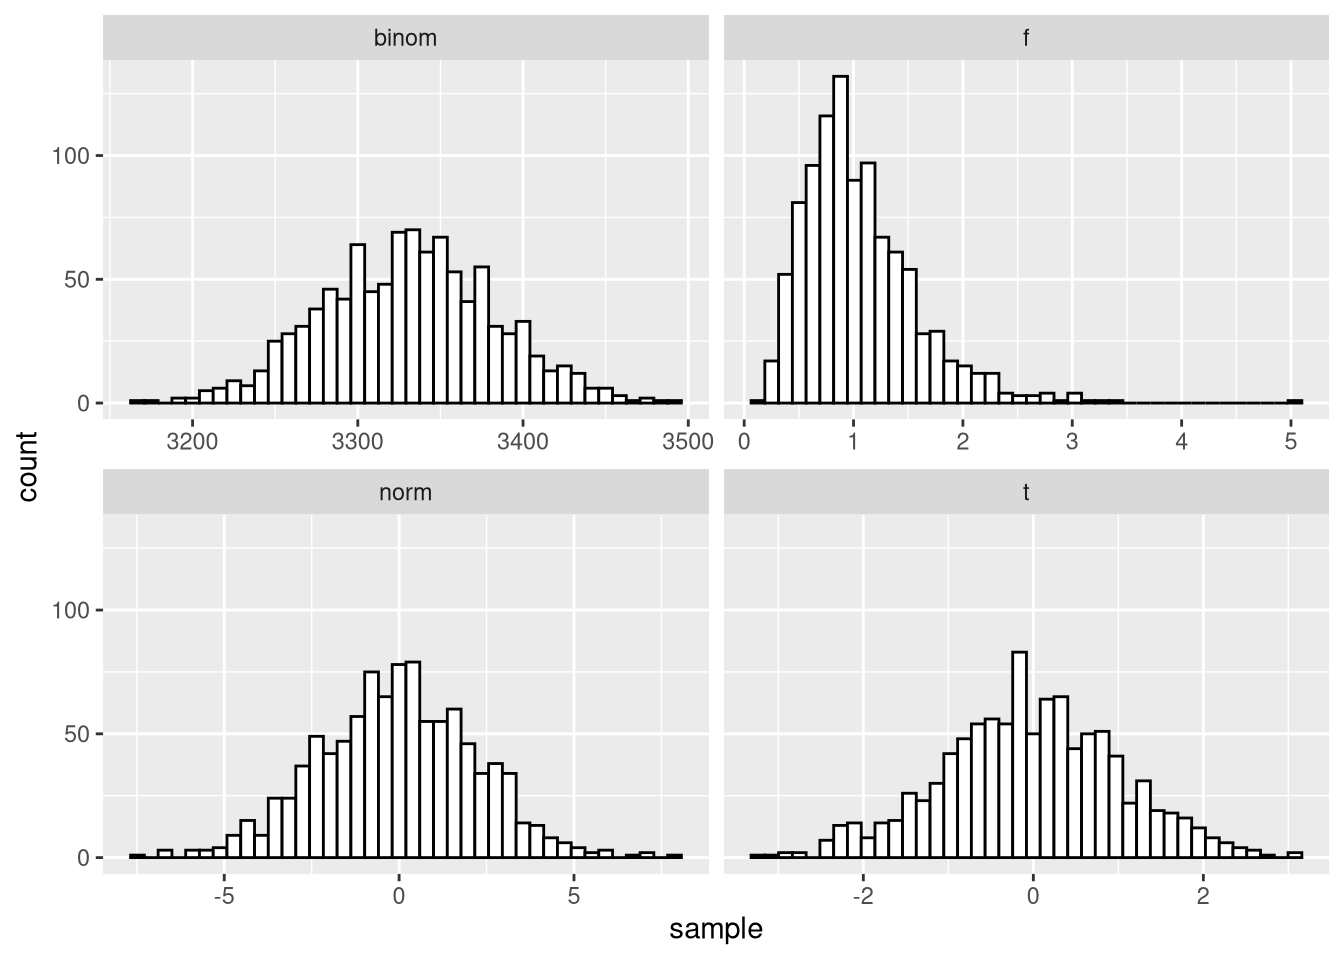
\includegraphics{Robustheit_files/figure-latex/unnamed-chunk-32-1.pdf}

\hypertarget{aufgabe-3}{%
\subsection{Aufgabe}\label{aufgabe-3}}

Erstelle eine Funktion \texttt{gen\_distributed\_values}, die mit Hilfe von \texttt{if}-Statements anhand eines Arguments \texttt{distribution} und eines Arguments \texttt{n} einen Vektor an Zufallszahlen generiert. Dabei soll \texttt{distribution} angeben, welche aus drei möglichen Verteilungen genutzt wird. Denke außerdem an mögliche Verteilungseigenschaften der genutzten Funktionen und füge sie als optionale Argumente zur Funktion hinzu.

Antwort

\begin{Shaded}
\begin{Highlighting}[]
\NormalTok{gen\_distributed\_values }\OtherTok{\textless{}{-}} \ControlFlowTok{function}\NormalTok{(distribution,}
\NormalTok{                                   n,}
                                   \AttributeTok{df =} \DecValTok{1}\NormalTok{,}
                                   \AttributeTok{lambda =} \DecValTok{25}\NormalTok{,}
                                   \AttributeTok{rate =} \DecValTok{5}\NormalTok{) \{}
  \ControlFlowTok{if}\NormalTok{(distribution }\SpecialCharTok{==} \StringTok{\textquotesingle{}t\textquotesingle{}}\NormalTok{)\{}
    \FunctionTok{return}\NormalTok{(}\FunctionTok{rt}\NormalTok{(n, df))}
\NormalTok{  \}}\ControlFlowTok{else} \ControlFlowTok{if}\NormalTok{(distribution }\SpecialCharTok{==} \StringTok{\textquotesingle{}pois\textquotesingle{}}\NormalTok{)\{}
    \FunctionTok{return}\NormalTok{(}\FunctionTok{rpois}\NormalTok{(n, lambda))}
\NormalTok{  \}}\ControlFlowTok{else} \ControlFlowTok{if}\NormalTok{(distribution }\SpecialCharTok{==} \StringTok{\textquotesingle{}exp\textquotesingle{}}\NormalTok{)\{}
    \FunctionTok{return}\NormalTok{(}\FunctionTok{rexp}\NormalTok{(n, rate))}
\NormalTok{  \}}
  \FunctionTok{print}\NormalTok{(}\StringTok{\textquotesingle{}Distribution is not implemented, returning zeros\textquotesingle{}}\NormalTok{)}
  \FunctionTok{return}\NormalTok{(}\FunctionTok{numeric}\NormalTok{(n))}
\NormalTok{\}}

\FunctionTok{gen\_distributed\_values}\NormalTok{(}\StringTok{\textquotesingle{}pois\textquotesingle{}}\NormalTok{,}
                       \DecValTok{5}\NormalTok{,}
                       \AttributeTok{lambda =} \DecValTok{3}\NormalTok{)}
\end{Highlighting}
\end{Shaded}

\begin{verbatim}
## [1] 4 4 3 5 2
\end{verbatim}

\hypertarget{schleifen}{%
\chapter{Schleifen}\label{schleifen}}

Bei so gut wie allen Simulationsproblemen stehen wir vor der Situation, dass wir eine Operation, zum Beispiel das Generieren einer gewissen Zahl an Zufallswerten und die Berechnung der zugehörigen Teststatistik, mehrere hundert Mal ausführen wollen.

Wir könnten jetzt die Operation mehrere hundert mal in unser Skript schreiben, damit würden wir aber zum Einen Fehler einladen, zum Anderen viel zu viel Lebenszeit verschwenden.

Deswegen gibt es in so gut wie jeder Programmiersprache irgendeine Form von Ausdrücken, die eine \emph{iterative} Wiederholung eines Ausdrucks ermöglichen.

Ein Beispiel für die Anweisung einer solchen iterativen Wiederholung sind Schleifen.
In R gibt es davon drei Arten:

\begin{itemize}
\item
  \texttt{repeat} - die flexibelste Schleife, die so lange wiederholt bis sie mit \texttt{break} unterbrochen wird
\item
  \texttt{while} - eine Schleife, die zu Beginn jeder Wiederholung einen logischen Test durchführt und bei Zutreffen die Operation wiederholt
\item
  \texttt{for} - die unflexibelste der drei Möglichkeiten. \texttt{for} iteriert einen Wert durch einen Vektor oder eine Liste, bis alle Einträge einmal dran waren. Das heißt, dass wir eine feste Laufzeit und damit den einfachsten Umgang haben, weswegen wir auch \texttt{for} in diesem Kurs verwenden werden.
\end{itemize}

Die \texttt{for}-Syntax sieht dabei wie folgt aus:

\begin{Shaded}
\begin{Highlighting}[]
\ControlFlowTok{for}\NormalTok{(value }\ControlFlowTok{in}\NormalTok{ vector)\{}
\NormalTok{  do something}
\NormalTok{\}}
\end{Highlighting}
\end{Shaded}

Um jetzt Beispielsweise alle Werte von eins bis zehn durch zu laufen und jeden Wert auszugeben können wir den folgenden Ausdruck benutzen:

\begin{Shaded}
\begin{Highlighting}[]
\ControlFlowTok{for}\NormalTok{(i }\ControlFlowTok{in} \FunctionTok{seq\_len}\NormalTok{(}\DecValTok{10}\NormalTok{))\{}
  \FunctionTok{print}\NormalTok{(i)}
\NormalTok{\}}
\end{Highlighting}
\end{Shaded}

\begin{verbatim}
## [1] 1
## [1] 2
## [1] 3
## [1] 4
## [1] 5
## [1] 6
## [1] 7
## [1] 8
## [1] 9
## [1] 10
\end{verbatim}

Wie man an diesem Beispiel schon sehen kann, können wir in der Schleife auf den \texttt{i}-Wert zugreifen. Das können wir zum Beispiel benutzen, um die ersten zehn Zahlen der Fibonacci-Reihe zu berechnen, in der jeder Wert die Summe der zwei vorhergegangenen ist:

\begin{Shaded}
\begin{Highlighting}[]
\NormalTok{fib }\OtherTok{\textless{}{-}} \FunctionTok{numeric}\NormalTok{(}\DecValTok{10}\NormalTok{)}
\ControlFlowTok{for}\NormalTok{(i }\ControlFlowTok{in} \FunctionTok{seq\_along}\NormalTok{(fib))\{}
  \ControlFlowTok{if}\NormalTok{(i}\SpecialCharTok{\textless{}}\DecValTok{3}\NormalTok{)\{ }\CommentTok{\# die ersten zwei Stellen müssen Einsen sein}
\NormalTok{    fib[i] }\OtherTok{\textless{}{-}} \DecValTok{1}
\NormalTok{  \}}\ControlFlowTok{else}\NormalTok{\{}
\NormalTok{    fib[i] }\OtherTok{\textless{}{-}}\NormalTok{ fib[i}\DecValTok{{-}1}\NormalTok{] }\SpecialCharTok{+}\NormalTok{ fib[i}\DecValTok{{-}2}\NormalTok{] }\CommentTok{\# nimm die letzten zwei Einträge und summier sie auf}
\NormalTok{  \}}
\NormalTok{\}}
\NormalTok{fib}
\end{Highlighting}
\end{Shaded}

\begin{verbatim}
##  [1]  1  1  2  3  5  8 13 21 34 55
\end{verbatim}

In diesem Beispiel ist noch ein weiteres Programmier-Prinzip sichtbar, die \emph{Allokation} des Ergebnis-Vektors vor der Berechnung der Werte. Damit ist einfach gemeint, dass wir den leeren \texttt{fib}-Vektor erstellt haben, bevor wir mit der Schleife angefangen haben.

Der Grund für dieses Vorgehen ist, dass jedes Anlegen eines Vektors einer bestimtmen Größe ein bisschen Rechenzeit kostet. Wenn wir von vornherein festlegen, wie lang der Vektor werden soll, müssen wir nur einen Vektor anlegen. Wenn wir stattdessen wie im folgenden Beispiel in jeder Iteration den Vektor vergrößern, erstellt R implizit in jeder Iteration einen neuen Vektor.

\begin{Shaded}
\begin{Highlighting}[]
\NormalTok{fib }\OtherTok{\textless{}{-}} \DecValTok{1}
\ControlFlowTok{for}\NormalTok{(i }\ControlFlowTok{in} \FunctionTok{seq\_len}\NormalTok{(}\DecValTok{10}\NormalTok{))\{}
  \ControlFlowTok{if}\NormalTok{(i}\SpecialCharTok{\textless{}}\DecValTok{3}\NormalTok{)\{ }
\NormalTok{    fib[i] }\OtherTok{\textless{}{-}} \DecValTok{1}
\NormalTok{  \}}\ControlFlowTok{else}\NormalTok{\{}
\NormalTok{    fib[i] }\OtherTok{\textless{}{-}}\NormalTok{ fib[i}\DecValTok{{-}1}\NormalTok{] }\SpecialCharTok{+}\NormalTok{ fib[i}\DecValTok{{-}2}\NormalTok{] }
\NormalTok{  \}}
\NormalTok{\}}
\NormalTok{fib}
\end{Highlighting}
\end{Shaded}

\begin{verbatim}
##  [1]  1  1  2  3  5  8 13 21 34 55
\end{verbatim}

Bei 10 Stellen ist der Unterschied noch nicht wirklich bemerkbar. Wenn wir jetzt aber das ganze in Funktionen verpacken und für längere Sequenzen laufen lassen und die Laufzeit stoppen sehen wir den Unterschied:

\begin{Shaded}
\begin{Highlighting}[]
\NormalTok{fib\_alloc }\OtherTok{\textless{}{-}} \ControlFlowTok{function}\NormalTok{(n)\{}
\NormalTok{  fib }\OtherTok{\textless{}{-}} \FunctionTok{numeric}\NormalTok{(n)}
  \ControlFlowTok{for}\NormalTok{(i }\ControlFlowTok{in} \FunctionTok{seq\_along}\NormalTok{(fib))\{}
    \ControlFlowTok{if}\NormalTok{(i}\SpecialCharTok{\textless{}}\DecValTok{3}\NormalTok{)\{ }
\NormalTok{      fib[i] }\OtherTok{\textless{}{-}} \DecValTok{1}
\NormalTok{    \}}\ControlFlowTok{else}\NormalTok{\{}
\NormalTok{      fib[i] }\OtherTok{\textless{}{-}}\NormalTok{ fib[i}\DecValTok{{-}1}\NormalTok{] }\SpecialCharTok{+}\NormalTok{ fib[i}\DecValTok{{-}2}\NormalTok{] }
\NormalTok{    \}}
\NormalTok{  \}}
  \FunctionTok{return}\NormalTok{(fib)}
\NormalTok{\}}


\NormalTok{fib\_no\_alloc }\OtherTok{\textless{}{-}} \ControlFlowTok{function}\NormalTok{(n)\{}
\NormalTok{  fib }\OtherTok{\textless{}{-}} \DecValTok{1}
  \ControlFlowTok{for}\NormalTok{(i }\ControlFlowTok{in} \FunctionTok{seq\_len}\NormalTok{(n))\{}
    \ControlFlowTok{if}\NormalTok{(i}\SpecialCharTok{\textless{}}\DecValTok{3}\NormalTok{)\{ }
\NormalTok{      fib[i] }\OtherTok{\textless{}{-}} \DecValTok{1}
\NormalTok{    \}}\ControlFlowTok{else}\NormalTok{\{}
\NormalTok{      fib[i] }\OtherTok{\textless{}{-}}\NormalTok{ fib[i}\DecValTok{{-}1}\NormalTok{] }\SpecialCharTok{+}\NormalTok{ fib[i}\DecValTok{{-}2}\NormalTok{] }
\NormalTok{    \}}
\NormalTok{  \}}
  \FunctionTok{return}\NormalTok{(fib)}
\NormalTok{\}}
\NormalTok{start }\OtherTok{\textless{}{-}} \FunctionTok{Sys.time}\NormalTok{()}
\NormalTok{a }\OtherTok{\textless{}{-}} \FunctionTok{fib\_alloc}\NormalTok{(}\DecValTok{100000}\NormalTok{)}
\NormalTok{runtime\_alloc }\OtherTok{\textless{}{-}} \FunctionTok{Sys.time}\NormalTok{() }\SpecialCharTok{{-}}\NormalTok{ start}
\NormalTok{start }\OtherTok{\textless{}{-}} \FunctionTok{Sys.time}\NormalTok{()}
\NormalTok{b }\OtherTok{\textless{}{-}} \FunctionTok{fib\_no\_alloc}\NormalTok{(}\DecValTok{100000}\NormalTok{)}
\NormalTok{runtime\_no\_alloc }\OtherTok{\textless{}{-}} \FunctionTok{Sys.time}\NormalTok{() }\SpecialCharTok{{-}}\NormalTok{ start}

\NormalTok{runtime\_alloc}
\end{Highlighting}
\end{Shaded}

\begin{verbatim}
## Time difference of 0.03702068 secs
\end{verbatim}

\begin{Shaded}
\begin{Highlighting}[]
\NormalTok{runtime\_no\_alloc}
\end{Highlighting}
\end{Shaded}

\begin{verbatim}
## Time difference of 0.08719563 secs
\end{verbatim}

Mehr als die Hälfte der Zeit geht für das Erstellen des neuen Vektors drauf!

\hypertarget{aufgabe-4}{%
\subsection{Aufgabe}\label{aufgabe-4}}

In QM-2 habt Ihr im Rahmen des zentralen Grenzwertsatzes gelernt, dass die Verteilungsfunktion der z-Transformation der n-ten Summe einer Reihe von unabhängigen Zufallsvariablen für wachsendes n schwach gegen die Standardnormalverteilung konvergiert.

Schreibe eine Funktion, die für eine gegebene Anzahl an Summen und eine gegebene Verteilungsklasse (und den entsprechenden Parametern inklusive der Stichprobengröße) einen Vektor mit den entsprechenden Summen zurückgibt.
Nutze dafür deine Funktion aus der letzten Aufgabe.

Nutze diese Funktion dann um ein Histogramm mit 5000 dieser z-transformierten Summen zu erstellen.

Antwort

\begin{Shaded}
\begin{Highlighting}[]
\NormalTok{gen\_central\_lim\_vec }\OtherTok{\textless{}{-}} \ControlFlowTok{function}\NormalTok{(N, }
\NormalTok{                                distribution,}
\NormalTok{                                n,}
                                \AttributeTok{df =} \DecValTok{1}\NormalTok{,}
                                \AttributeTok{lambda =} \DecValTok{25}\NormalTok{,}
                                \AttributeTok{rate =} \DecValTok{5}\NormalTok{) \{}
  
\NormalTok{  ret\_vec }\OtherTok{\textless{}{-}} \FunctionTok{numeric}\NormalTok{(N)}
  \ControlFlowTok{for}\NormalTok{(i }\ControlFlowTok{in} \FunctionTok{seq\_len}\NormalTok{(N))\{}
\NormalTok{    ret\_vec[i] }\OtherTok{\textless{}{-}} \FunctionTok{sum}\NormalTok{(}\FunctionTok{gen\_distributed\_values}\NormalTok{(distribution,}
\NormalTok{                                      n,}
\NormalTok{                                      df,}
\NormalTok{                                      lambda,}
\NormalTok{                                      rate))}
\NormalTok{  \}}
  \FunctionTok{return}\NormalTok{(ret\_vec)}
\NormalTok{\}}

\FunctionTok{tibble}\NormalTok{(}\AttributeTok{sample =} \FunctionTok{scale}\NormalTok{(}\FunctionTok{gen\_central\_lim\_vec}\NormalTok{(}\DecValTok{5000}\NormalTok{, }\StringTok{\textquotesingle{}exp\textquotesingle{}}\NormalTok{, }\DecValTok{1000}\NormalTok{,}\AttributeTok{rate =} \DecValTok{5}\NormalTok{))) }\SpecialCharTok{\%\textgreater{}\%} 
  \FunctionTok{ggplot}\NormalTok{(}\FunctionTok{aes}\NormalTok{(}\AttributeTok{x =}\NormalTok{ sample)) }\SpecialCharTok{+}
  \FunctionTok{geom\_histogram}\NormalTok{(}\AttributeTok{binwidth =}\NormalTok{ .}\DecValTok{1}\NormalTok{,}
                 \AttributeTok{color =} \StringTok{\textquotesingle{}grey\textquotesingle{}}\NormalTok{,}
                 \AttributeTok{fill =} \StringTok{\textquotesingle{}white\textquotesingle{}}\NormalTok{)}
\end{Highlighting}
\end{Shaded}

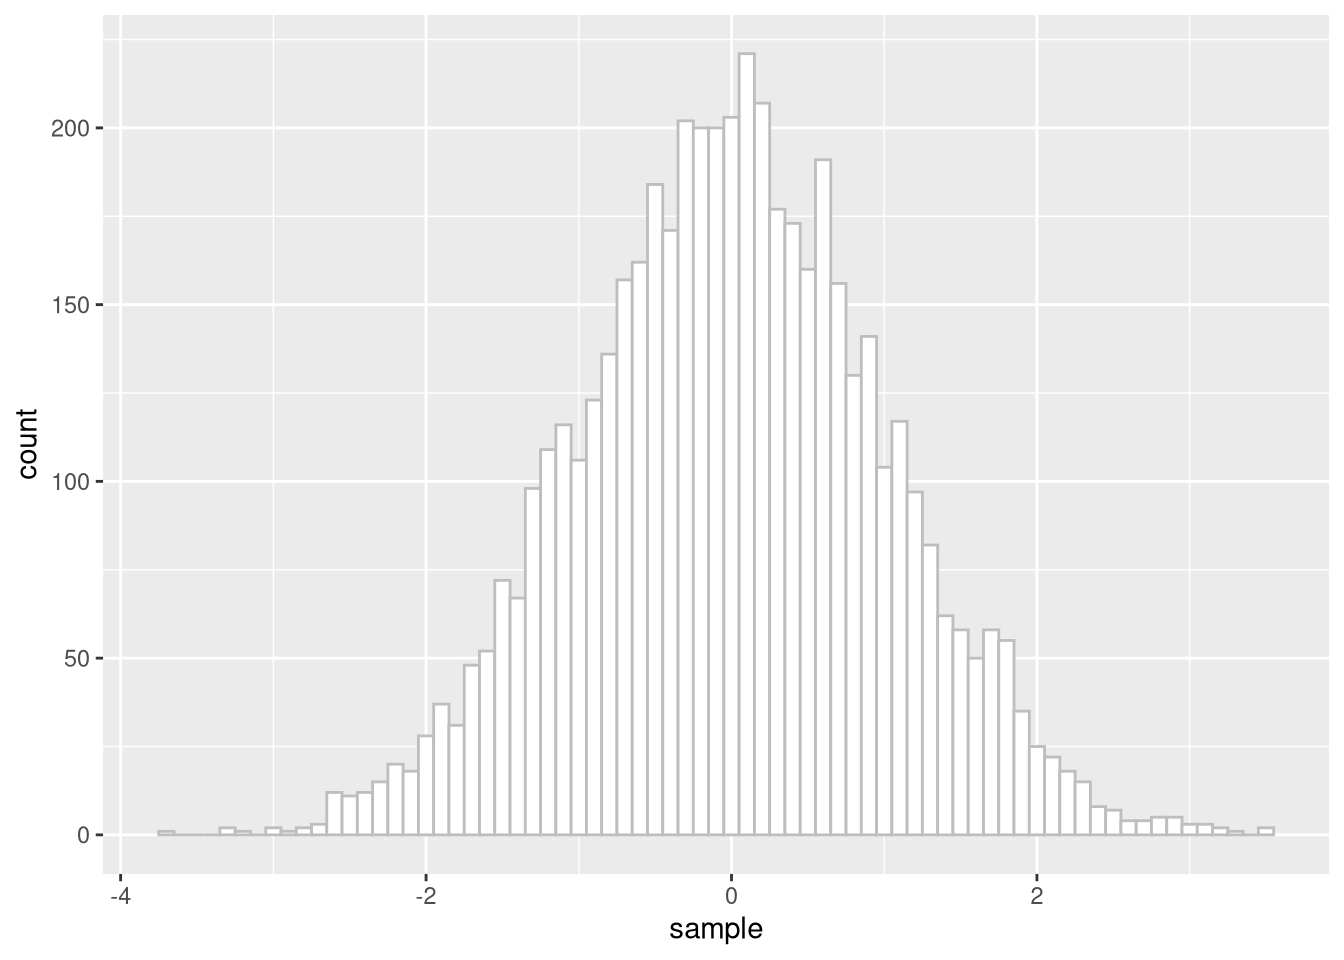
\includegraphics{Robustheit_files/figure-latex/unnamed-chunk-39-1.pdf}

\hypertarget{listen}{%
\chapter{Listen}\label{listen}}

Listen sind uns aus der R-Übung schon im Rahmen der \href{https://mbrede.github.io/CAU_Kiel_EDVI/aggregation-und-filemanagement.html\#lazy-evaluation}{Gruppenweisen Aggregation mit \texttt{across}} und \href{https://mbrede.github.io/CAU_KIEL_EDVII/einfache-lineare-zusammenh\%C3\%A4nge.html\#weitere-parameter}{als Output von Inferenzstatistischen Funktionen} untergekommen.
Aber was genau Listen architektonisch sind, haben wir bisher übergangen.

Listen sind in R ziemlich ähnlich zu Vektoren \footnote{Wobei der Ausdruck ``Vektoren'' hier irreführend ist, in R wird eigentlich die Eltern-Klasse der Objekte \texttt{Vector} genannt, zu der \texttt{Atomic}(unsere ``Vektoren'') und \texttt{List} gehören. Da wir aber in den Grundlagenfächern wegen der mathematischen Analogie ``Vektor'' zu den \texttt{Atomic}-Objekten gesagt haben, behalten wir das hier bei.}. Sie bilden Aneinander-Kettungen von Objekten ab, bei denen wir die einzelnen Elemente benennen können.
Ein Unterschied zu Vektoren ist aber, dass die Objekte nicht von einem einzelnen Typ sein müssen.
Ein anderer Unterschied wird deutlich, wenn wir uns den Output von benannten Vektoren und Listen genauer anschauen.

\begin{Shaded}
\begin{Highlighting}[]
\FunctionTok{c}\NormalTok{(}\StringTok{\textquotesingle{}a\textquotesingle{}}\OtherTok{=} \DecValTok{1}\NormalTok{,}
  \StringTok{\textquotesingle{}b\textquotesingle{}}\OtherTok{=} \DecValTok{2}\NormalTok{)}
\end{Highlighting}
\end{Shaded}

\begin{verbatim}
## a b 
## 1 2
\end{verbatim}

\begin{Shaded}
\begin{Highlighting}[]
\FunctionTok{list}\NormalTok{(}\StringTok{\textquotesingle{}a\textquotesingle{}}\OtherTok{=} \DecValTok{1}\NormalTok{,}
     \StringTok{\textquotesingle{}b\textquotesingle{}}\OtherTok{=} \DecValTok{2}\NormalTok{)}
\end{Highlighting}
\end{Shaded}

\begin{verbatim}
## $a
## [1] 1
## 
## $b
## [1] 2
\end{verbatim}

Die Ausgabe der Liste ähnelt unter der jeweiligen Überschrift (z.B.: \texttt{\$a}) dem Output, den wir bei einem unbenannten Vektor sehen:

\begin{Shaded}
\begin{Highlighting}[]
\FunctionTok{c}\NormalTok{(}\DecValTok{1}\NormalTok{)}
\end{Highlighting}
\end{Shaded}

\begin{verbatim}
## [1] 1
\end{verbatim}

Das liegt daran, dass in einer Liste unter dem Namen auch der ganze Vektor ``abgespeichert'' ist. Abgespeichert ist hier in Anführungszeichen, da in der Liste eigentlich nur ein Verweis auf einen Vektor liegt. Das kann man sich verdeutlichen, wenn man sich die Größen von Vektoren und Listen im Arbeitsspeicher anguckt.

Dazu erstellen wir einen Vektoren mit den Zahlen von 1:1000 und eine Liste, der wir dreimal diesen Vektor übergeben.

\begin{Shaded}
\begin{Highlighting}[]
\NormalTok{a }\OtherTok{\textless{}{-}} \FunctionTok{c}\NormalTok{(}\DecValTok{1}\SpecialCharTok{:}\DecValTok{1000}\NormalTok{)}

\NormalTok{b }\OtherTok{\textless{}{-}} \FunctionTok{list}\NormalTok{(}\AttributeTok{a =}\NormalTok{ a, }\AttributeTok{b =}\NormalTok{ a, }\AttributeTok{c =}\NormalTok{ a, }\AttributeTok{d =}\NormalTok{ a)}
\end{Highlighting}
\end{Shaded}

Wenn wir uns jetzt die Größen der beiden Objekte angucken, sehen wir dass die Liste kleiner ist, als vielleicht zuerst erwartet:

\begin{Shaded}
\begin{Highlighting}[]
\NormalTok{lobstr}\SpecialCharTok{::}\FunctionTok{obj\_size}\NormalTok{(a)}
\end{Highlighting}
\end{Shaded}

\begin{verbatim}
## 4,048 B
\end{verbatim}

\begin{Shaded}
\begin{Highlighting}[]
\NormalTok{lobstr}\SpecialCharTok{::}\FunctionTok{obj\_size}\NormalTok{(b)}
\end{Highlighting}
\end{Shaded}

\begin{verbatim}
## 4,544 B
\end{verbatim}

Wenn wir die Liste mit einem vergleichbaren Vektor gegenüberstellen sehen wir, dass dieser die Werte offensichtlich direkt ablegt, wohingegen die Liste die Werte nur einmal beinhaltet (plus ein bisschen Speicher für die wiederholten Verweise und Namen):

\begin{Shaded}
\begin{Highlighting}[]
\NormalTok{d }\OtherTok{\textless{}{-}} \FunctionTok{c}\NormalTok{(a, a, a, a)}

\NormalTok{lobstr}\SpecialCharTok{::}\FunctionTok{obj\_size}\NormalTok{(a)}
\end{Highlighting}
\end{Shaded}

\begin{verbatim}
## 4,048 B
\end{verbatim}

\begin{Shaded}
\begin{Highlighting}[]
\NormalTok{lobstr}\SpecialCharTok{::}\FunctionTok{obj\_size}\NormalTok{(b)}
\end{Highlighting}
\end{Shaded}

\begin{verbatim}
## 4,544 B
\end{verbatim}

\begin{Shaded}
\begin{Highlighting}[]
\NormalTok{lobstr}\SpecialCharTok{::}\FunctionTok{obj\_size}\NormalTok{(d)}
\end{Highlighting}
\end{Shaded}

\begin{verbatim}
## 16,048 B
\end{verbatim}

Was passiert nun, wenn wir einen Teil eines der vier Einträge in der Liste ändern?

Dazu können wir die schon von \texttt{data.frames} bekannte Index-Variante mit dem \texttt{\$}-Operator nutzen um einen der Vektoren in der Liste zu modifizieren:

\begin{Shaded}
\begin{Highlighting}[]
\NormalTok{b}\SpecialCharTok{$}\NormalTok{a[}\DecValTok{1}\NormalTok{] }\OtherTok{\textless{}{-}} \DecValTok{5}
\NormalTok{lobstr}\SpecialCharTok{::}\FunctionTok{obj\_size}\NormalTok{(b)}
\end{Highlighting}
\end{Shaded}

\begin{verbatim}
## 12,592 B
\end{verbatim}

Die Liste wird größer. Dass sie nicht in Inkrementen von 4000 B größer wird, liegt daran, dass die Zahlen in \texttt{a} als Sequenz von R effizienter gespeichert werden können, als als einfache Zahlen. Wenn wir uns \texttt{a} alleine angucken und die Größe vor und nach Änderung der ersten Stelle betrachten, wird das deutlich:

\begin{Shaded}
\begin{Highlighting}[]
\NormalTok{lobstr}\SpecialCharTok{::}\FunctionTok{obj\_size}\NormalTok{(a)}
\end{Highlighting}
\end{Shaded}

\begin{verbatim}
## 4,048 B
\end{verbatim}

\begin{Shaded}
\begin{Highlighting}[]
\NormalTok{a[}\DecValTok{1}\NormalTok{] }\OtherTok{\textless{}{-}} \DecValTok{5}

\NormalTok{lobstr}\SpecialCharTok{::}\FunctionTok{obj\_size}\NormalTok{(a)}
\end{Highlighting}
\end{Shaded}

\begin{verbatim}
## 8,048 B
\end{verbatim}

Für mehr Details zu diesem Speicher-Verhalten und dem zugrunde liegenden Prinzip ist das kostenlos \href{https://adv-r.hadley.nz/index.html}{hier zugängliche} Buch ``Advanced R'' \citet{wickhamAdvanced2019} sehr gut, vor allem die \href{https://adv-r.hadley.nz/names-values.html\#binding-basics}{Kapitel 2.2} und folgende und das \href{https://adv-r.hadley.nz/vectors-chap.html}{Kapitel über Vektoren}.

\hypertarget{aufgabe-5}{%
\subsubsection{Aufgabe}\label{aufgabe-5}}

Überlege dir, wie sich der Speicherbedarf der Liste \texttt{b} ändert, wenn Du den zweiten Platz der Liste mit dem ersten Platz der Liste überschreibst.
Probiere dann aus, ob sich deine Vorhersage bewahrheitet.
Überprüfe dann, was passiert, wenn du die erste Stelle des dritten Platzes der Liste durch fünf ersetzt.
Was könnte hier passiert sein?

Antwort

\begin{Shaded}
\begin{Highlighting}[]
\NormalTok{a }\OtherTok{\textless{}{-}} \FunctionTok{c}\NormalTok{(}\DecValTok{1}\SpecialCharTok{:}\DecValTok{1000}\NormalTok{)}
\NormalTok{b }\OtherTok{\textless{}{-}} \FunctionTok{list}\NormalTok{(}\AttributeTok{a =}\NormalTok{ a,}\AttributeTok{b =}\NormalTok{ a,}\AttributeTok{c =}\NormalTok{ a,}\AttributeTok{d =}\NormalTok{ a)}
\NormalTok{b}\SpecialCharTok{$}\NormalTok{a[}\DecValTok{1}\NormalTok{] }\OtherTok{\textless{}{-}} \DecValTok{5}
\NormalTok{lobstr}\SpecialCharTok{::}\FunctionTok{obj\_size}\NormalTok{(b)}
\end{Highlighting}
\end{Shaded}

\begin{verbatim}
## 12,592 B
\end{verbatim}

\begin{Shaded}
\begin{Highlighting}[]
\NormalTok{b}\SpecialCharTok{$}\NormalTok{b }\OtherTok{\textless{}{-}}\NormalTok{ b}\SpecialCharTok{$}\NormalTok{a}
\NormalTok{lobstr}\SpecialCharTok{::}\FunctionTok{obj\_size}\NormalTok{(b)}
\end{Highlighting}
\end{Shaded}

\begin{verbatim}
## 12,592 B
\end{verbatim}

\begin{Shaded}
\begin{Highlighting}[]
\NormalTok{b}\SpecialCharTok{$}\NormalTok{c[}\DecValTok{1}\NormalTok{] }\OtherTok{\textless{}{-}} \DecValTok{5}
\NormalTok{lobstr}\SpecialCharTok{::}\FunctionTok{obj\_size}\NormalTok{(b)}
\end{Highlighting}
\end{Shaded}

\begin{verbatim}
## 20,640 B
\end{verbatim}

\hypertarget{listen-und-datensuxe4tze}{%
\section{Listen und Datensätze}\label{listen-und-datensuxe4tze}}

Das Arbeiten mit Listen ist ziemlich ähnlich zu der mit Datensätzen.
Das liegt ganz einfach daran, dass Datensätze auch Listen sind, der einzige wirklich wichtige Unterschied ist, dass Datensätze im Vergleich zu Listen einheitliche Längen von den eingefügten Vektoren erwarten.

Zu sehen ist dieses Verhältnis ganz einfach, wenn man sich den \texttt{mode} eines Datensatzes anguckt:

\begin{Shaded}
\begin{Highlighting}[]
\NormalTok{a }\OtherTok{\textless{}{-}} \FunctionTok{data.frame}\NormalTok{(}\DecValTok{1}\SpecialCharTok{:}\DecValTok{10}\NormalTok{,}
                \DecValTok{1}\SpecialCharTok{:}\DecValTok{10}\NormalTok{)}

\FunctionTok{class}\NormalTok{(a)}
\end{Highlighting}
\end{Shaded}

\begin{verbatim}
## [1] "data.frame"
\end{verbatim}

\begin{Shaded}
\begin{Highlighting}[]
\FunctionTok{mode}\NormalTok{(a)}
\end{Highlighting}
\end{Shaded}

\begin{verbatim}
## [1] "list"
\end{verbatim}

Der Unterschied ist in den \texttt{attributes} des Datensatzes festgelegt.

\begin{Shaded}
\begin{Highlighting}[]
\FunctionTok{attributes}\NormalTok{(a)}
\end{Highlighting}
\end{Shaded}

\begin{verbatim}
## $names
## [1] "X1.10"   "X1.10.1"
## 
## $class
## [1] "data.frame"
## 
## $row.names
##  [1]  1  2  3  4  5  6  7  8  9 10
\end{verbatim}

Nur zum Spaß können wir so auch versuchen, umständlich einen Datensatz zu erstellen:

\begin{Shaded}
\begin{Highlighting}[]
\NormalTok{a }\OtherTok{\textless{}{-}} \FunctionTok{list}\NormalTok{(}\DecValTok{1}\SpecialCharTok{:}\DecValTok{10}\NormalTok{,}\DecValTok{1}\SpecialCharTok{:}\DecValTok{10}\NormalTok{)}
\FunctionTok{attributes}\NormalTok{(a)}
\end{Highlighting}
\end{Shaded}

\begin{verbatim}
## NULL
\end{verbatim}

\begin{Shaded}
\begin{Highlighting}[]
\FunctionTok{attributes}\NormalTok{(a) }\OtherTok{\textless{}{-}} \FunctionTok{list}\NormalTok{(}\AttributeTok{names =}\NormalTok{ letters[}\DecValTok{1}\SpecialCharTok{:}\DecValTok{2}\NormalTok{],}
                      \AttributeTok{row.names =} \DecValTok{1}\SpecialCharTok{:}\DecValTok{10}\NormalTok{,}
                      \AttributeTok{class =} \StringTok{"data.frame"}\NormalTok{)}
\NormalTok{a}
\end{Highlighting}
\end{Shaded}

\begin{verbatim}
##     a  b
## 1   1  1
## 2   2  2
## 3   3  3
## 4   4  4
## 5   5  5
## 6   6  6
## 7   7  7
## 8   8  8
## 9   9  9
## 10 10 10
\end{verbatim}

\hypertarget{aufgabe-6}{%
\subsubsection{Aufgabe}\label{aufgabe-6}}

Überlege Dir, was wohl passiert, wenn du auf die gerade demonstrierte Art und Weise einen Datensatz erstellst, bei dem die eingefügten Vektoren von unterschiedlicher Länge sind.
Überprüfe dann, ob die Erwartungen stimmen.

Antwort

\begin{Shaded}
\begin{Highlighting}[]
\NormalTok{a }\OtherTok{\textless{}{-}} \FunctionTok{list}\NormalTok{(}\DecValTok{1}\SpecialCharTok{:}\DecValTok{15}\NormalTok{,}\DecValTok{21}\SpecialCharTok{:}\DecValTok{30}\NormalTok{,}\DecValTok{41}\SpecialCharTok{:}\DecValTok{45}\NormalTok{)}
\FunctionTok{attributes}\NormalTok{(a)}
\end{Highlighting}
\end{Shaded}

\begin{verbatim}
## NULL
\end{verbatim}

\begin{Shaded}
\begin{Highlighting}[]
\FunctionTok{attributes}\NormalTok{(a) }\OtherTok{\textless{}{-}} \FunctionTok{list}\NormalTok{(}\AttributeTok{names =}\NormalTok{ letters[}\DecValTok{1}\SpecialCharTok{:}\DecValTok{3}\NormalTok{],}
                      \AttributeTok{row.names =} \DecValTok{1}\SpecialCharTok{:}\DecValTok{10}\NormalTok{,}
                      \AttributeTok{class =} \StringTok{"data.frame"}\NormalTok{)}
\NormalTok{a}
\end{Highlighting}
\end{Shaded}

\begin{verbatim}
## Warning in format.data.frame(if (omit) x[seq_len(n0), , drop = FALSE] else x, :
## corrupt data frame: columns will be truncated or padded with NAs
\end{verbatim}

\begin{verbatim}
##     a  b    c
## 1   1 21   41
## 2   2 22   42
## 3   3 23   43
## 4   4 24   44
## 5   5 25   45
## 6   6 26 <NA>
## 7   7 27 <NA>
## 8   8 28 <NA>
## 9   9 29 <NA>
## 10 10 30 <NA>
\end{verbatim}

\hypertarget{arbeiten-mit-listen}{%
\section{Arbeiten mit Listen}\label{arbeiten-mit-listen}}

Da Datensätze eigentlich nur Listen sind, gibt es Listen-Operationen die wir schon von Datensätzen kennen, bei denen wir einfach noch nicht wussten, dass sie eigentlich aus dem Listen-Kontext stammen.

Insbesondere sind die Operationen, die wir auch schon hier im Skript genutzt haben, Listen-Operationen, die wir aus dem \texttt{data.frame}-Kontext kennen.
Da wären das Anlegen von Spalten/Listen-Einträgen mit Namen, wie wir es eben gesehen haben:

\begin{Shaded}
\begin{Highlighting}[]
\NormalTok{a }\OtherTok{\textless{}{-}} \FunctionTok{list}\NormalTok{(}\AttributeTok{a =} \DecValTok{1}\SpecialCharTok{:}\DecValTok{10}\NormalTok{)}
\NormalTok{b }\OtherTok{\textless{}{-}} \FunctionTok{data.frame}\NormalTok{(}\AttributeTok{a =} \DecValTok{1}\SpecialCharTok{:}\DecValTok{10}\NormalTok{)}
\end{Highlighting}
\end{Shaded}

Und das Indizieren mit dem \texttt{\$}-Operator:

\begin{Shaded}
\begin{Highlighting}[]
\NormalTok{a}\SpecialCharTok{$}\NormalTok{a}
\end{Highlighting}
\end{Shaded}

\begin{verbatim}
##  [1]  1  2  3  4  5  6  7  8  9 10
\end{verbatim}

\begin{Shaded}
\begin{Highlighting}[]
\NormalTok{b}\SpecialCharTok{$}\NormalTok{a}
\end{Highlighting}
\end{Shaded}

\begin{verbatim}
##  [1]  1  2  3  4  5  6  7  8  9 10
\end{verbatim}

Als kleinen Zusatz können wir uns noch die numerische Indizierung angucken, die bei Listen und damit auch Datensätzen mit doppelten eckigen Klammern funktioniert (\texttt{{[}{[}{]}{]}}). Dieser Index-Operator ist hilfreich, wenn nicht jedes mal für jeden Eintrag ein Name angelegt werden soll. Das kann zum Beispiel sinnvoll bei \texttt{functional}-Iteratoren sein, bei denen man nur eine schnelle Stapelverarbeitung plant, dazu aber später mehr.

Bei Listen und Datensätzen sieht der \texttt{{[}{[}{]}{]}}-Einsatz dann so aus:

\begin{Shaded}
\begin{Highlighting}[]
\NormalTok{a[[}\DecValTok{1}\NormalTok{]]}
\end{Highlighting}
\end{Shaded}

\begin{verbatim}
##  [1]  1  2  3  4  5  6  7  8  9 10
\end{verbatim}

\begin{Shaded}
\begin{Highlighting}[]
\NormalTok{b[[}\DecValTok{1}\NormalTok{]]}
\end{Highlighting}
\end{Shaded}

\begin{verbatim}
##  [1]  1  2  3  4  5  6  7  8  9 10
\end{verbatim}

\hypertarget{aufgabe-7}{%
\subsubsection{Aufgabe}\label{aufgabe-7}}

Baue ein Skript, das eine Liste erstellt, die drei Einträge enthält.
Jeder dieser Einträge soll auch wieder eine Liste sein.
Das Skript soll nun mit Hilfe einer Schleife die Zahlen von 1 bis 100 durchgehen und alle durch 2 teilbaren Zahlen in den zweiten Eintrag, alle durch 3 teilbaren Zahlen in den dritten Eintrag und alle restlichen Zahlen in den ersten Eintrag einfügen.
Nutze hierfür den ``Modulo''-Operator \texttt{\%\%}, der den `Rest' einer Ganzzahldivision ausgibt.
Überlege dir, wie du mit Zahlen wie der 6 umgehst, die sowohl durch 3 als auch durch 2 teilbar sind.
Kleiner Tipp: \texttt{length} kann hier sehr hilfreich sein.

Zusatzaufgabe:
Überlege dir, wie man dieses Skript so umbauen könnte, dass es für einen Vektor mit beliebigen Teilern funktioniert.

Antwort

\begin{Shaded}
\begin{Highlighting}[]
\NormalTok{divisions }\OtherTok{\textless{}{-}} \FunctionTok{list}\NormalTok{(}\FunctionTok{list}\NormalTok{(), }\FunctionTok{list}\NormalTok{(), }\FunctionTok{list}\NormalTok{())}

\ControlFlowTok{for}\NormalTok{(i }\ControlFlowTok{in} \DecValTok{1}\SpecialCharTok{:}\DecValTok{100}\NormalTok{)\{}
  \ControlFlowTok{if}\NormalTok{(i}\SpecialCharTok{\%\%}\DecValTok{2} \SpecialCharTok{==} \DecValTok{0}\NormalTok{)\{}
\NormalTok{    divisions[[}\DecValTok{2}\NormalTok{]][[}\FunctionTok{length}\NormalTok{(divisions[[}\DecValTok{2}\NormalTok{]]) }\SpecialCharTok{+} \DecValTok{1}\NormalTok{]] }\OtherTok{\textless{}{-}}\NormalTok{ i}
\NormalTok{  \}}
  \ControlFlowTok{if}\NormalTok{(i}\SpecialCharTok{\%\%}\DecValTok{3} \SpecialCharTok{==} \DecValTok{0}\NormalTok{)\{}
\NormalTok{    divisions[[}\DecValTok{3}\NormalTok{]][[}\FunctionTok{length}\NormalTok{(divisions[[}\DecValTok{3}\NormalTok{]]) }\SpecialCharTok{+} \DecValTok{1}\NormalTok{]] }\OtherTok{\textless{}{-}}\NormalTok{ i}
\NormalTok{  \}}
  \ControlFlowTok{if}\NormalTok{(i}\SpecialCharTok{\%\%}\DecValTok{2} \SpecialCharTok{!=} \DecValTok{0} \SpecialCharTok{\&}\NormalTok{ i}\SpecialCharTok{\%\%}\DecValTok{3} \SpecialCharTok{!=} \DecValTok{0}\NormalTok{)\{}
\NormalTok{    divisions[[}\DecValTok{1}\NormalTok{]][[}\FunctionTok{length}\NormalTok{(divisions[[}\DecValTok{1}\NormalTok{]]) }\SpecialCharTok{+} \DecValTok{1}\NormalTok{]] }\OtherTok{\textless{}{-}}\NormalTok{ i}
\NormalTok{  \}}
\NormalTok{\}}
\FunctionTok{summary}\NormalTok{(divisions)}
\end{Highlighting}
\end{Shaded}

\begin{verbatim}
##      Length Class  Mode
## [1,] 33     -none- list
## [2,] 50     -none- list
## [3,] 33     -none- list
\end{verbatim}

\begin{Shaded}
\begin{Highlighting}[]
\DocumentationTok{\#\# Zusatz:}
\NormalTok{divisions }\OtherTok{\textless{}{-}} \FunctionTok{list}\NormalTok{(}\FunctionTok{list}\NormalTok{()) }\CommentTok{\# mit einer leeren Liste für die nicht{-}teilbaren initiieren}
\NormalTok{divider }\OtherTok{\textless{}{-}} \FunctionTok{c}\NormalTok{(}\DecValTok{2}\NormalTok{,}\DecValTok{3}\NormalTok{,}\DecValTok{5}\NormalTok{,}\DecValTok{7}\NormalTok{,}\DecValTok{9}\NormalTok{)}
\ControlFlowTok{for}\NormalTok{(i }\ControlFlowTok{in}\NormalTok{ divider)\{}
\NormalTok{  divisions[[i]] }\OtherTok{\textless{}{-}} \FunctionTok{list}\NormalTok{()}
\NormalTok{\}}
\ControlFlowTok{for}\NormalTok{(i }\ControlFlowTok{in} \DecValTok{1}\SpecialCharTok{:}\DecValTok{100}\NormalTok{)\{}
\NormalTok{  divided }\OtherTok{\textless{}{-}}\NormalTok{  F}
  \ControlFlowTok{for}\NormalTok{(j }\ControlFlowTok{in}\NormalTok{ divider)\{}
    \ControlFlowTok{if}\NormalTok{(i }\SpecialCharTok{\%\%}\NormalTok{ j }\SpecialCharTok{==} \DecValTok{0}\NormalTok{)\{}
\NormalTok{      divisions[[j]][[}\FunctionTok{length}\NormalTok{(divisions[[j]]) }\SpecialCharTok{+} \DecValTok{1}\NormalTok{]] }\OtherTok{\textless{}{-}}\NormalTok{ i}
\NormalTok{      divided }\OtherTok{\textless{}{-}}\NormalTok{ T}
\NormalTok{    \}}
\NormalTok{  \}}
  \ControlFlowTok{if}\NormalTok{(}\SpecialCharTok{!}\NormalTok{divided)\{}
\NormalTok{    divisions[[}\DecValTok{1}\NormalTok{]][[}\FunctionTok{length}\NormalTok{(divisions[[}\DecValTok{1}\NormalTok{]]) }\SpecialCharTok{+} \DecValTok{1}\NormalTok{]] }\OtherTok{\textless{}{-}}\NormalTok{ i}
\NormalTok{  \}}
\NormalTok{\}}

\FunctionTok{summary}\NormalTok{(divisions)}
\end{Highlighting}
\end{Shaded}

\begin{verbatim}
##       Length Class  Mode
##  [1,] 22     -none- list
##  [2,] 50     -none- list
##  [3,] 33     -none- list
##  [4,]  0     -none- NULL
##  [5,] 20     -none- list
##  [6,]  0     -none- NULL
##  [7,] 14     -none- list
##  [8,]  0     -none- NULL
##  [9,] 11     -none- list
\end{verbatim}

\begin{Shaded}
\begin{Highlighting}[]
\FunctionTok{unlist}\NormalTok{(divisions[[}\DecValTok{1}\NormalTok{]]) }\CommentTok{\# Mit Teilern und ohne 1 haben wir hier die Primzahlen bis 100 gesammelt.}
\end{Highlighting}
\end{Shaded}

\begin{verbatim}
##  [1]  1 11 13 17 19 23 29 31 37 41 43 47 53 59 61 67 71 73 79 83 89 97
\end{verbatim}

\hypertarget{attribute}{%
\chapter{Attribute}\label{attribute}}

Bei der sehr umständlichen Erstellung des Datensatzes haben wir schon die \texttt{attributes} kennen gelernt. Diese Informationen, die in R zu einem Objekt neben dem eigentlichen Inhalt angelegt werden können, sind ein wichtiger Teil der Abbildung objektorientierter Programmierparadigmen\footnote{Was genau objektorientierte Programmierung ist, ist hier erstmal nicht so wichtig, im Prinzip sind aber alle Objekte mit \texttt{class}-Attribut nach objektorientierten Paradigmen erstellt. Hier wird das nur erwähnt, weil es die Geschichte von R als Nachfolger von S demonstriert, in dem ursprünglich ``moderne'' Paradigmen nicht Thema waren. Die Erweiterung der bestehenden Objekte durch das Setzen von Attributen ist die Lösung für dieses Problem, die in Rs \texttt{S3}-Objekten resultieren. Daneben gibt es in R die \texttt{S4}-Objekte, die formalisiertere Klassendefinitionen ermöglichen. Das führt aber alles ein bisschen weit für diese Veranstaltung, deswegen sei hier nochmal auf das sehr gute Buch von \citet{wickhamAdvanced2019} verwiesen, in den Kapiteln 13-15 geht er auf OO-Programmierung in R ein.} in R.

\begin{Shaded}
\begin{Highlighting}[]
\NormalTok{a }\OtherTok{\textless{}{-}} \FunctionTok{list}\NormalTok{(}\DecValTok{1}\SpecialCharTok{:}\DecValTok{10}\NormalTok{,}\DecValTok{1}\SpecialCharTok{:}\DecValTok{10}\NormalTok{)}
\FunctionTok{attributes}\NormalTok{(a)}
\end{Highlighting}
\end{Shaded}

\begin{verbatim}
## NULL
\end{verbatim}

\begin{Shaded}
\begin{Highlighting}[]
\FunctionTok{attributes}\NormalTok{(a) }\OtherTok{\textless{}{-}} \FunctionTok{list}\NormalTok{(}\AttributeTok{names =}\NormalTok{ letters[}\DecValTok{1}\SpecialCharTok{:}\DecValTok{2}\NormalTok{],}
                      \AttributeTok{row.names =} \DecValTok{1}\SpecialCharTok{:}\DecValTok{10}\NormalTok{,}
                      \AttributeTok{class =} \StringTok{"data.frame"}\NormalTok{)}
\NormalTok{a}
\end{Highlighting}
\end{Shaded}

\begin{verbatim}
##     a  b
## 1   1  1
## 2   2  2
## 3   3  3
## 4   4  4
## 5   5  5
## 6   6  6
## 7   7  7
## 8   8  8
## 9   9  9
## 10 10 10
\end{verbatim}

Neben der Klasse (\texttt{class}) haben wir hier in die \texttt{attributes} auch die Namen der Einträge und die Zeilennamen geschrieben. Wir sehen also, dass der sichtbare und bemerkbare Unterschied zwischen Listen und Datensätzen aus dem Setzen dieser Attribute entsteht. Außerdem wird an diesem Beispiel deutlich, dass die Funktionen, die wir bisher zum Erstellen von Datensätzen genutzt haben, auch eigentlich nur Attribute setzen.
Attribute sind also zusätzliche Informationen, die den Umgang mit Objekten ändern können.

Ein weiteres Beispiel für solche Änderungen durch Attribute sind Matritzen. In R kann man mit der \texttt{matrix}-Funktion zweidimensionale Daten-Raster erstellen, für die zum Beispiel auch die dimensionierte Indizierung \texttt{{[},{]}} definiert ist:

\begin{Shaded}
\begin{Highlighting}[]
\FunctionTok{matrix}\NormalTok{(}\DecValTok{1}\SpecialCharTok{:}\DecValTok{100}\NormalTok{,}
       \AttributeTok{nrow =} \DecValTok{10}\NormalTok{, }
       \AttributeTok{ncol =} \DecValTok{10}\NormalTok{)}
\end{Highlighting}
\end{Shaded}

\begin{verbatim}
##       [,1] [,2] [,3] [,4] [,5] [,6] [,7] [,8] [,9] [,10]
##  [1,]    1   11   21   31   41   51   61   71   81    91
##  [2,]    2   12   22   32   42   52   62   72   82    92
##  [3,]    3   13   23   33   43   53   63   73   83    93
##  [4,]    4   14   24   34   44   54   64   74   84    94
##  [5,]    5   15   25   35   45   55   65   75   85    95
##  [6,]    6   16   26   36   46   56   66   76   86    96
##  [7,]    7   17   27   37   47   57   67   77   87    97
##  [8,]    8   18   28   38   48   58   68   78   88    98
##  [9,]    9   19   29   39   49   59   69   79   89    99
## [10,]   10   20   30   40   50   60   70   80   90   100
\end{verbatim}

\hypertarget{aufgabe-8}{%
\subsubsection{Aufgabe}\label{aufgabe-8}}

Erstelle eine Matrix und gucke die genau die Attribute und Inhalte an.

Können wir so wie wir einen Datensatz aus einer Liste erstellt haben, irgendwie ohne die \texttt{matrix}-Funktion eine Matrix erstellen? Gucke Dir dabei nach jeder Änderung an, was \texttt{class} und \texttt{mode} zurückgeben.

Probiere außerdem aus, was passiert, wenn man die Attribute einer Matrix auf eine Liste überträgt.

\textbf{Zusatz:}

Was passiert, wenn wir der Liste drei Dimensionen geben?

Antwort

\begin{Shaded}
\begin{Highlighting}[]
\NormalTok{my\_mat }\OtherTok{\textless{}{-}} \FunctionTok{matrix}\NormalTok{(letters[}\DecValTok{1}\SpecialCharTok{:}\DecValTok{20}\NormalTok{],}
                 \DecValTok{4}\NormalTok{)}

\FunctionTok{attributes}\NormalTok{(my\_mat)}
\end{Highlighting}
\end{Shaded}

\begin{verbatim}
## $dim
## [1] 4 5
\end{verbatim}

\begin{Shaded}
\begin{Highlighting}[]
\FunctionTok{mode}\NormalTok{(my\_mat)}
\end{Highlighting}
\end{Shaded}

\begin{verbatim}
## [1] "character"
\end{verbatim}

\begin{Shaded}
\begin{Highlighting}[]
\FunctionTok{class}\NormalTok{(my\_mat)}
\end{Highlighting}
\end{Shaded}

\begin{verbatim}
## [1] "matrix" "array"
\end{verbatim}

\begin{Shaded}
\begin{Highlighting}[]
\NormalTok{my\_list\_mat }\OtherTok{\textless{}{-}} \FunctionTok{list}\NormalTok{(}\DecValTok{1}\SpecialCharTok{:}\DecValTok{5}\NormalTok{,}\DecValTok{6}\SpecialCharTok{:}\DecValTok{10}\NormalTok{,}\DecValTok{11}\SpecialCharTok{:}\DecValTok{15}\NormalTok{,}\DecValTok{16}\SpecialCharTok{:}\DecValTok{20}\NormalTok{)}

\FunctionTok{attributes}\NormalTok{(my\_list\_mat) }\OtherTok{\textless{}{-}} \FunctionTok{list}\NormalTok{(}\AttributeTok{dim =} \FunctionTok{c}\NormalTok{(}\DecValTok{2}\NormalTok{,}\DecValTok{2}\NormalTok{))}
\NormalTok{my\_list\_mat}
\end{Highlighting}
\end{Shaded}

\begin{verbatim}
##      [,1]      [,2]     
## [1,] integer,5 integer,5
## [2,] integer,5 integer,5
\end{verbatim}

\begin{Shaded}
\begin{Highlighting}[]
\FunctionTok{mode}\NormalTok{(my\_list\_mat)}
\end{Highlighting}
\end{Shaded}

\begin{verbatim}
## [1] "list"
\end{verbatim}

\begin{Shaded}
\begin{Highlighting}[]
\FunctionTok{class}\NormalTok{(my\_list\_mat)}
\end{Highlighting}
\end{Shaded}

\begin{verbatim}
## [1] "matrix" "array"
\end{verbatim}

\begin{Shaded}
\begin{Highlighting}[]
\DocumentationTok{\#\# Zusatz}
\NormalTok{my\_list\_mat }\OtherTok{\textless{}{-}} \FunctionTok{list}\NormalTok{(}\DecValTok{1}\NormalTok{, }\DecValTok{2}\NormalTok{, }
                    \DecValTok{3}\NormalTok{, }\DecValTok{4}\NormalTok{, }
                    \DecValTok{5}\NormalTok{, }\DecValTok{6}\NormalTok{, }
                    \DecValTok{7}\NormalTok{, }\DecValTok{8}\NormalTok{)}

\FunctionTok{attributes}\NormalTok{(my\_list\_mat) }\OtherTok{\textless{}{-}} \FunctionTok{list}\NormalTok{(}\AttributeTok{dim =} \FunctionTok{c}\NormalTok{(}\DecValTok{2}\NormalTok{,}\DecValTok{4}\NormalTok{))}
\NormalTok{my\_list\_mat}
\end{Highlighting}
\end{Shaded}

\begin{verbatim}
##      [,1] [,2] [,3] [,4]
## [1,] 1    3    5    7   
## [2,] 2    4    6    8
\end{verbatim}

\begin{Shaded}
\begin{Highlighting}[]
\FunctionTok{mode}\NormalTok{(my\_list\_mat)}
\end{Highlighting}
\end{Shaded}

\begin{verbatim}
## [1] "list"
\end{verbatim}

\begin{Shaded}
\begin{Highlighting}[]
\FunctionTok{class}\NormalTok{(my\_list\_mat)}
\end{Highlighting}
\end{Shaded}

\begin{verbatim}
## [1] "matrix" "array"
\end{verbatim}

\begin{Shaded}
\begin{Highlighting}[]
\FunctionTok{attributes}\NormalTok{(my\_list\_mat) }\OtherTok{\textless{}{-}} \FunctionTok{list}\NormalTok{(}\AttributeTok{dim =} \FunctionTok{c}\NormalTok{(}\DecValTok{2}\NormalTok{,}\DecValTok{2}\NormalTok{,}\DecValTok{2}\NormalTok{))}
\NormalTok{my\_list\_mat}
\end{Highlighting}
\end{Shaded}

\begin{verbatim}
## , , 1
## 
##      [,1] [,2]
## [1,] 1    3   
## [2,] 2    4   
## 
## , , 2
## 
##      [,1] [,2]
## [1,] 5    7   
## [2,] 6    8
\end{verbatim}

\begin{Shaded}
\begin{Highlighting}[]
\FunctionTok{mode}\NormalTok{(my\_list\_mat)}
\end{Highlighting}
\end{Shaded}

\begin{verbatim}
## [1] "list"
\end{verbatim}

\begin{Shaded}
\begin{Highlighting}[]
\FunctionTok{class}\NormalTok{(my\_list\_mat)}
\end{Highlighting}
\end{Shaded}

\begin{verbatim}
## [1] "array"
\end{verbatim}

Mit anderen Worten ist eine Matrix als ein Array definiert, das (egal ob Liste oder Vektor), zwei Dimensionen hat. Mit mehr als zwei Dimensionen fällt die Matrix-Klasse weg.

Die Matrix-Listen aus der Aufgabe können wir übrigens auch wie Matrizen verwenden:

\begin{Shaded}
\begin{Highlighting}[]
\FunctionTok{attributes}\NormalTok{(my\_list\_mat) }\OtherTok{\textless{}{-}} \FunctionTok{list}\NormalTok{(}\AttributeTok{dim =} \FunctionTok{c}\NormalTok{(}\DecValTok{2}\NormalTok{,}\DecValTok{4}\NormalTok{))}

\FunctionTok{t}\NormalTok{(my\_list\_mat)}
\end{Highlighting}
\end{Shaded}

\begin{verbatim}
##      [,1] [,2]
## [1,] 1    2   
## [2,] 3    4   
## [3,] 5    6   
## [4,] 7    8
\end{verbatim}

\begin{Shaded}
\begin{Highlighting}[]
\NormalTok{my\_list\_mat[}\DecValTok{1}\NormalTok{,}\DecValTok{2}\NormalTok{]}
\end{Highlighting}
\end{Shaded}

\begin{verbatim}
## [[1]]
## [1] 3
\end{verbatim}

Das Ergebnis ist halt nur eine Liste, was mit dem bekannten doppel-Index aber auch umgangen werden kann:

\begin{Shaded}
\begin{Highlighting}[]
\NormalTok{my\_list\_mat[[}\DecValTok{1}\NormalTok{,}\DecValTok{2}\NormalTok{]]}
\end{Highlighting}
\end{Shaded}

\begin{verbatim}
## [1] 3
\end{verbatim}

\hypertarget{functionals}{%
\chapter{Functionals}\label{functionals}}

Wie wir am Anfang des Semesters bei der Definition unserer eigenen Funktionen ja schon gemerkt haben, sind Funktionen in R von der Struktur her gar nicht so verschieden zu anderen Objekten wie zum Beispiel Datensätzen oder Vektoren.

Sowohl die einen, wie auch die anderen, werden als Namen mit entsprechenden Inhalten im Environment angelegt, wobei aber natürlich bei Datensätzen die Daten damit gemeint sind und bei Funktionen \emph{Environment}-Verweis, \emph{Body} und \emph{Formals} angelegt werden.

Das heißt für R aber auch, dass so genannte \emph{Functionals} genutzt werden. Diese Gruppe von Funktionen sind solche, die andere Funktionen als Argumente und diese anwenden können. Beispiele für solche Funktionen haben wir auch schon kennen gelernt, die vielleicht aus dem Kapitel zur \href{https://mbrede.github.io/CAU_Kiel_EDVI/aggregation-und-filemanagement.html}{Aggregation} von Daten in EDV1 bekannte \texttt{across}-Funktion ist ein solcher Fall:

\begin{Shaded}
\begin{Highlighting}[]
\NormalTok{iris }\SpecialCharTok{\%\textgreater{}\%} 
  \FunctionTok{group\_by}\NormalTok{(Species) }\SpecialCharTok{\%\textgreater{}\%} 
  \FunctionTok{summarise}\NormalTok{(}\FunctionTok{across}\NormalTok{(}\FunctionTok{where}\NormalTok{(is.numeric),}
                   \AttributeTok{.fns =} \FunctionTok{list}\NormalTok{(}\AttributeTok{m =}\NormalTok{ mean, }\AttributeTok{s =}\NormalTok{ sd),}
                   \AttributeTok{.names =} \StringTok{\textquotesingle{}\{.fn\}\_\{.col\}\textquotesingle{}}\NormalTok{))}
\end{Highlighting}
\end{Shaded}

\begin{verbatim}
## # A tibble: 3 x 9
##   Species    m_Sepal.Length s_Sepal.Length m_Sepal.Width s_Sepal.Width
##   <fct>               <dbl>          <dbl>         <dbl>         <dbl>
## 1 setosa               5.01          0.352          3.43         0.379
## 2 versicolor           5.94          0.516          2.77         0.314
## 3 virginica            6.59          0.636          2.97         0.322
## # ... with 4 more variables: m_Petal.Length <dbl>, s_Petal.Length <dbl>,
## #   m_Petal.Width <dbl>, s_Petal.Width <dbl>
\end{verbatim}

Hier übergeben wir dem \texttt{.fns}-Argument eine Liste mit Funktionen, die dann auf alle numerischen Spalten des Datensatzes angewandt werden.

Ein anderes, sehr für R typisches Beispiel von Functionals sind \texttt{sapply}, \texttt{lapply} und \texttt{mapply}. Alle drei Funktionen nehmen als Input eins oder mehrere Objekte und eine Funktion, die auf jeden Eintrag de(s/r) übergebenen Objekte(s) angewandt werden soll.

Exemplarisch gucken wir uns \texttt{sapply} an, die Listen\footnote{oder Vektoren} als erstes Argument erwarten.
Als Objekt nehmen wir \texttt{iris} (was ja wie wir gelernt habe eine aufgemotzte Liste ist) und lassen uns mit \texttt{sapply} für jede Spalte sagen, ob sie numerisch ist:

\begin{Shaded}
\begin{Highlighting}[]
\FunctionTok{sapply}\NormalTok{(iris, is.numeric)}
\end{Highlighting}
\end{Shaded}

\begin{verbatim}
## Sepal.Length  Sepal.Width Petal.Length  Petal.Width      Species 
##         TRUE         TRUE         TRUE         TRUE        FALSE
\end{verbatim}

Fällt Dir was auf?
Wir haben gerade eine Funktion fünf mal ausgeführt, ohne ihr explizit ein Argument zu übergeben. Den (\texttt{is.numeric(iris\$Sepal.Width)},\texttt{is.numeric(iris\$Sepal.Length)}, etc., etc., \ldots)-Teil hat uns \texttt{sapply} abgenommen. \texttt{sapply} ist sogar so weit gegangen, uns die Ergebnisse in einem praktischen Vektor wiederzugeben, hat also irgendwie einen Output für uns erstellt.

Diesen Vektor könnten wir jetzt als Index nutzen, um uns nur die numerischen Spalten ausgeben zu lassen und uns wieder mit \texttt{sapply} die Mittelwerte ausrechnen zu lassen:

\begin{Shaded}
\begin{Highlighting}[]
\FunctionTok{sapply}\NormalTok{(iris[,}\FunctionTok{which}\NormalTok{(}\FunctionTok{sapply}\NormalTok{(iris, is.numeric))],}
\NormalTok{       mean)}
\end{Highlighting}
\end{Shaded}

\begin{verbatim}
## Sepal.Length  Sepal.Width Petal.Length  Petal.Width 
##     5.843333     3.057333     3.758000     1.199333
\end{verbatim}

Die \texttt{sapply}-Funktion macht also im Prinzip nicht viel anderes, als unsere \texttt{for}-Schleifen.

\hypertarget{aufgabe-9}{%
\subsection{Aufgabe}\label{aufgabe-9}}

Baue die oben mit \texttt{sapply} implementierte Mittlung mit \texttt{for}-Schleifen nach.
Dabei soll erst überprüft werden, ob eine Spalte numerische Inhalte hat, wenn dem so ist soll der Mittelwert dieser Spalte berechnet werden.
Verpacke deine Lösung in eine Funktion, die den spaltenweisen Mittelwert zurückgibt.

Überlege dir insbesondere, ob Du den Output-Vektor allozieren kannst und was ein sinnvolles Format dafür wäre.

Antwort

\begin{Shaded}
\begin{Highlighting}[]
\NormalTok{my\_col\_mean }\OtherTok{\textless{}{-}} \ControlFlowTok{function}\NormalTok{(df)\{}
\NormalTok{  out }\OtherTok{\textless{}{-}} \FunctionTok{rep}\NormalTok{(}\ConstantTok{NA}\NormalTok{, }\FunctionTok{ncol}\NormalTok{(df))}
  \FunctionTok{names}\NormalTok{(out) }\OtherTok{\textless{}{-}} \FunctionTok{names}\NormalTok{(df)}
  \ControlFlowTok{for}\NormalTok{(col }\ControlFlowTok{in} \FunctionTok{names}\NormalTok{(df))\{}
    \ControlFlowTok{if}\NormalTok{(}\FunctionTok{is.numeric}\NormalTok{(df[[col]]))\{}
\NormalTok{      out[col] }\OtherTok{\textless{}{-}} \FunctionTok{mean}\NormalTok{(df[[col]])}
\NormalTok{    \}}
\NormalTok{  \}}
  \FunctionTok{return}\NormalTok{(out)}
\NormalTok{\}}
\FunctionTok{my\_col\_mean}\NormalTok{(iris)}
\end{Highlighting}
\end{Shaded}

\begin{verbatim}
## Sepal.Length  Sepal.Width Petal.Length  Petal.Width      Species 
##     5.843333     3.057333     3.758000     1.199333           NA
\end{verbatim}

\hypertarget{purrrmap}{%
\section{\texorpdfstring{\texttt{purrr::map}}{purrr::map}}\label{purrrmap}}

Eine Alternative zu den \texttt{*apply}-Funktionen ist die \texttt{map}-Familie aus dem \texttt{purrr}-Paket. Im Prinzip sind die identisch zu den \texttt{*apply}-Funktionen, der große Unterschied ist, dass sie spezialisierter sind als erstere.

Diese Eigenschaft ist auch der einzige wirkliche Grund dafür, die functional-Iteratoren den Schleifen vorzuziehen. Code, der so spezifisch für ein Problem wie möglich ist, ist einfach schöner weil schneller verständlich.

Die grundlegende Funktion aus der \texttt{map}-Familie ist das einfache \texttt{map}, das \texttt{lapply}-Analogon. \texttt{map} nimmt also eine Liste oder einen Vektor und eine Funktion als Input und gibt eine Liste zurück:

\begin{Shaded}
\begin{Highlighting}[]
\FunctionTok{map}\NormalTok{(}\DecValTok{1}\SpecialCharTok{:}\DecValTok{10}\NormalTok{, sqrt)}
\end{Highlighting}
\end{Shaded}

\begin{verbatim}
## [[1]]
## [1] 1
## 
## [[2]]
## [1] 1.414214
## 
## [[3]]
## [1] 1.732051
## 
## [[4]]
## [1] 2
## 
## [[5]]
## [1] 2.236068
## 
## [[6]]
## [1] 2.44949
## 
## [[7]]
## [1] 2.645751
## 
## [[8]]
## [1] 2.828427
## 
## [[9]]
## [1] 3
## 
## [[10]]
## [1] 3.162278
\end{verbatim}

Alternativ kann mit der sogenannten Funktionsschreibweise auch ein Ausdruck formuliert werden, der für jeden iterierten Wert ausgeführt werden soll:

\begin{Shaded}
\begin{Highlighting}[]
\FunctionTok{map\_dbl}\NormalTok{(}\DecValTok{1}\SpecialCharTok{:}\DecValTok{10}\NormalTok{, }\SpecialCharTok{\textasciitilde{}}\FunctionTok{sqrt}\NormalTok{(.))}
\end{Highlighting}
\end{Shaded}

\begin{verbatim}
##  [1] 1.000000 1.414214 1.732051 2.000000 2.236068 2.449490 2.645751 2.828427
##  [9] 3.000000 3.162278
\end{verbatim}

Der besondere Vorteil dieser Funktionen gegenüber den \texttt{*apply}-Funktionen, ist die Gruppe von Funktionen, die klar lesbar den erwarteten Output einer Iteration definieren.

Beispielsweise kann mit \texttt{map\_dbl}, \texttt{map\_lgl} und \texttt{map\_chr} klar festgelegt werden, dass 1. ein \texttt{atomic}-Vektor ausgegeben wird, der 2. einen klaren Datentyp hat:

\begin{Shaded}
\begin{Highlighting}[]
\FunctionTok{map\_dbl}\NormalTok{(}\DecValTok{1}\SpecialCharTok{:}\DecValTok{10}\NormalTok{, }\SpecialCharTok{\textasciitilde{}}\NormalTok{.}\SpecialCharTok{\^{}}\DecValTok{2}\NormalTok{)}
\end{Highlighting}
\end{Shaded}

\begin{verbatim}
##  [1]   1   4   9  16  25  36  49  64  81 100
\end{verbatim}

\begin{Shaded}
\begin{Highlighting}[]
\FunctionTok{map\_lgl}\NormalTok{(}\DecValTok{1}\SpecialCharTok{:}\DecValTok{10}\NormalTok{, }\SpecialCharTok{\textasciitilde{}}\NormalTok{.}\SpecialCharTok{\%\%}\DecValTok{2}\SpecialCharTok{==}\DecValTok{0}\NormalTok{)}
\end{Highlighting}
\end{Shaded}

\begin{verbatim}
##  [1] FALSE  TRUE FALSE  TRUE FALSE  TRUE FALSE  TRUE FALSE  TRUE
\end{verbatim}

\begin{Shaded}
\begin{Highlighting}[]
\FunctionTok{map\_chr}\NormalTok{(}\DecValTok{1}\SpecialCharTok{:}\DecValTok{10}\NormalTok{, }\SpecialCharTok{\textasciitilde{}}\NormalTok{letters[.])}
\end{Highlighting}
\end{Shaded}

\begin{verbatim}
##  [1] "a" "b" "c" "d" "e" "f" "g" "h" "i" "j"
\end{verbatim}

Und, noch praktischer, auch für komplexere Datentypen gibt es Wrapper. So können wir zum Beispiel mit \texttt{map\_dfr} und \texttt{map\_dfc} \texttt{tibble}s erzeugen lassen, die dann aus zeilenweise (\texttt{df}\emph{\texttt{r}} für rows) und spaltenweise (\texttt{df}\emph{\texttt{c}} für columns) zusammengefügten Ergebnissen bestehen:

\begin{Shaded}
\begin{Highlighting}[]
\FunctionTok{map\_dfr}\NormalTok{(}\DecValTok{1}\SpecialCharTok{:}\DecValTok{10}\NormalTok{, }\SpecialCharTok{\textasciitilde{}}\FunctionTok{tibble}\NormalTok{(}\AttributeTok{i =}\NormalTok{ .,}
                      \AttributeTok{x =} \FunctionTok{sample}\NormalTok{(}\DecValTok{1}\SpecialCharTok{:}\DecValTok{10}\NormalTok{,}\DecValTok{1}\NormalTok{)))}
\end{Highlighting}
\end{Shaded}

\begin{verbatim}
## # A tibble: 10 x 2
##        i     x
##    <int> <int>
##  1     1    10
##  2     2     7
##  3     3     3
##  4     4     5
##  5     5     3
##  6     6     7
##  7     7     5
##  8     8    10
##  9     9     1
## 10    10     3
\end{verbatim}

\begin{Shaded}
\begin{Highlighting}[]
\FunctionTok{map\_dfc}\NormalTok{(}\DecValTok{1}\SpecialCharTok{:}\DecValTok{10}\NormalTok{, }\SpecialCharTok{\textasciitilde{}}\FunctionTok{c}\NormalTok{(}\FunctionTok{sample}\NormalTok{(.}\SpecialCharTok{:}\NormalTok{(.}\SpecialCharTok{+}\DecValTok{10}\NormalTok{),}\DecValTok{1}\NormalTok{)))}
\end{Highlighting}
\end{Shaded}

\begin{verbatim}
## New names:
## * NA -> ...1
## * NA -> ...2
## * NA -> ...3
## * NA -> ...4
## * NA -> ...5
## * ...
\end{verbatim}

\begin{verbatim}
## # A tibble: 1 x 10
##    ...1  ...2  ...3  ...4  ...5  ...6  ...7  ...8  ...9 ...10
##   <int> <int> <int> <int> <int> <int> <int> <int> <int> <int>
## 1     5     8     3     4    15     9    11    15    13    10
\end{verbatim}

\hypertarget{exkurs-iteratoren-vergleich}{%
\section{Exkurs: Iteratoren-Vergleich}\label{exkurs-iteratoren-vergleich}}

Man liest manchmal, dass loops in R wegen geringerer Geschwindigkeit in jedem Fall vermieden werden sollten. Das stimmt aber nicht wirklich, wenn man für seine \texttt{for}-Schleifen alloziert.

Um das zu zeigen vergleichen wir mit der folgenden Funktion \texttt{for} ohne Allokation, for mit Allokation, \texttt{sapply} und \texttt{map\_dbl}:

\begin{Shaded}
\begin{Highlighting}[]
\NormalTok{my\_function }\OtherTok{\textless{}{-}} \ControlFlowTok{function}\NormalTok{(x) x}\SpecialCharTok{\^{}}\DecValTok{2}



\NormalTok{my\_test }\OtherTok{\textless{}{-}} \ControlFlowTok{function}\NormalTok{(i)\{}
\NormalTok{  out }\OtherTok{\textless{}{-}} \FunctionTok{list}\NormalTok{()}
\NormalTok{  out[[}\StringTok{\textquotesingle{}len\textquotesingle{}}\NormalTok{]] }\OtherTok{\textless{}{-}} \DecValTok{10}\SpecialCharTok{\^{}}\NormalTok{(i}\SpecialCharTok{\%\%}\DecValTok{6}\NormalTok{)}
\NormalTok{  to\_do }\OtherTok{\textless{}{-}} \DecValTok{1}\SpecialCharTok{:}\NormalTok{out[[}\StringTok{\textquotesingle{}len\textquotesingle{}}\NormalTok{]]}
\NormalTok{  start }\OtherTok{\textless{}{-}} \FunctionTok{Sys.time}\NormalTok{()}
\NormalTok{  res }\OtherTok{\textless{}{-}} \FunctionTok{c}\NormalTok{()}
  \ControlFlowTok{for}\NormalTok{(j }\ControlFlowTok{in}\NormalTok{ to\_do)\{}
\NormalTok{    res }\OtherTok{\textless{}{-}} \FunctionTok{c}\NormalTok{(res, }\FunctionTok{my\_function}\NormalTok{(j))}
\NormalTok{  \}}
\NormalTok{  out[[}\StringTok{\textquotesingle{}for ohne Allokation\textquotesingle{}}\NormalTok{]] }\OtherTok{\textless{}{-}} \FunctionTok{Sys.time}\NormalTok{() }\SpecialCharTok{{-}}\NormalTok{ start}
  
\NormalTok{  start }\OtherTok{\textless{}{-}} \FunctionTok{Sys.time}\NormalTok{()}
\NormalTok{  res }\OtherTok{\textless{}{-}} \FunctionTok{numeric}\NormalTok{(}\FunctionTok{length}\NormalTok{(to\_do))}
  \ControlFlowTok{for}\NormalTok{(j }\ControlFlowTok{in}\NormalTok{ to\_do)\{}
\NormalTok{    res[j] }\OtherTok{\textless{}{-}} \FunctionTok{my\_function}\NormalTok{(j)}
\NormalTok{  \}}
\NormalTok{  out[[}\StringTok{\textquotesingle{}for mit Allokation\textquotesingle{}}\NormalTok{]] }\OtherTok{\textless{}{-}} \FunctionTok{Sys.time}\NormalTok{() }\SpecialCharTok{{-}}\NormalTok{ start}
  
\NormalTok{  start }\OtherTok{\textless{}{-}} \FunctionTok{Sys.time}\NormalTok{()}
\NormalTok{  res }\OtherTok{\textless{}{-}} \FunctionTok{sapply}\NormalTok{(to\_do, my\_function)}
\NormalTok{  out[[}\StringTok{\textquotesingle{}sapply\textquotesingle{}}\NormalTok{]] }\OtherTok{\textless{}{-}} \FunctionTok{Sys.time}\NormalTok{() }\SpecialCharTok{{-}}\NormalTok{ start}
  
\NormalTok{  start }\OtherTok{\textless{}{-}} \FunctionTok{Sys.time}\NormalTok{()}
\NormalTok{  res }\OtherTok{\textless{}{-}} \FunctionTok{map\_dbl}\NormalTok{(to\_do, my\_function)}
\NormalTok{  out[[}\StringTok{\textquotesingle{}map\_dbl\textquotesingle{}}\NormalTok{]] }\OtherTok{\textless{}{-}} \FunctionTok{Sys.time}\NormalTok{() }\SpecialCharTok{{-}}\NormalTok{ start}
  \FunctionTok{return}\NormalTok{(out)}
\NormalTok{\}}
\end{Highlighting}
\end{Shaded}

\hypertarget{aufgabe-10}{%
\subsection{Aufgabe}\label{aufgabe-10}}

Was passiert hier?

Antwort

\begin{Shaded}
\begin{Highlighting}[]
\NormalTok{my\_function }\OtherTok{\textless{}{-}} \ControlFlowTok{function}\NormalTok{(x) x}\SpecialCharTok{\^{}}\DecValTok{2} \CommentTok{\# Funktion zum Quadrieren}

\NormalTok{my\_test }\OtherTok{\textless{}{-}} \ControlFlowTok{function}\NormalTok{(i)\{}
\NormalTok{  out }\OtherTok{\textless{}{-}} \FunctionTok{list}\NormalTok{() }\CommentTok{\# initiiere leere output{-}Liste}
\NormalTok{  out[[}\StringTok{\textquotesingle{}len\textquotesingle{}}\NormalTok{]] }\OtherTok{\textless{}{-}} \DecValTok{10}\SpecialCharTok{\^{}}\NormalTok{(i}\SpecialCharTok{\%\%}\DecValTok{6}\NormalTok{) }\CommentTok{\# Berechne Länge der Iteration als }
  \CommentTok{\# 10{-}Potenz zwischen 0 und 5}
\NormalTok{  to\_do }\OtherTok{\textless{}{-}} \DecValTok{1}\SpecialCharTok{:}\NormalTok{out[[}\StringTok{\textquotesingle{}len\textquotesingle{}}\NormalTok{]] }\CommentTok{\# durch zu iterierender Vektor}
\NormalTok{  start }\OtherTok{\textless{}{-}} \FunctionTok{Sys.time}\NormalTok{() }\CommentTok{\# Startzeit erster Test}
\NormalTok{  res }\OtherTok{\textless{}{-}} \FunctionTok{c}\NormalTok{() }\CommentTok{\# initiiere leeren Vektor (keine Allokation)}
  \ControlFlowTok{for}\NormalTok{(j }\ControlFlowTok{in}\NormalTok{ to\_do)\{ }\CommentTok{\# iteriere duch to\_do}
\NormalTok{    res }\OtherTok{\textless{}{-}} \FunctionTok{c}\NormalTok{(res, }\FunctionTok{my\_function}\NormalTok{(j)) }\CommentTok{\#quadriere jede Zahl und }
    \CommentTok{\# vergrößere res mit jeder Iteration}
\NormalTok{  \}}
\NormalTok{  out[[}\StringTok{\textquotesingle{}for ohne Allokation\textquotesingle{}}\NormalTok{]] }\OtherTok{\textless{}{-}} \FunctionTok{Sys.time}\NormalTok{() }\SpecialCharTok{{-}}\NormalTok{ start }\CommentTok{\# berechne Zeit{-}delta}
  
\NormalTok{  start }\OtherTok{\textless{}{-}} \FunctionTok{Sys.time}\NormalTok{() }\CommentTok{\# Startzeit zweiter Test}
\NormalTok{  res }\OtherTok{\textless{}{-}} \FunctionTok{numeric}\NormalTok{(}\FunctionTok{length}\NormalTok{(to\_do))}\CommentTok{\# initiiere Vektor mit Allokation}
  \ControlFlowTok{for}\NormalTok{(j }\ControlFlowTok{in}\NormalTok{ to\_do)\{}\CommentTok{\# iteriere durch to\_do}
\NormalTok{    res[j] }\OtherTok{\textless{}{-}} \FunctionTok{my\_function}\NormalTok{(j) }\CommentTok{\#quadriere jede Zahl und lege in res ab}
\NormalTok{  \}}
\NormalTok{  out[[}\StringTok{\textquotesingle{}for mit Allokation\textquotesingle{}}\NormalTok{]] }\OtherTok{\textless{}{-}} \FunctionTok{Sys.time}\NormalTok{() }\SpecialCharTok{{-}}\NormalTok{ start }\CommentTok{\# berechne Zeit{-}delta}
  
\NormalTok{  start }\OtherTok{\textless{}{-}} \FunctionTok{Sys.time}\NormalTok{() }\CommentTok{\# Startzeit dritter Test}
\NormalTok{  res }\OtherTok{\textless{}{-}} \FunctionTok{sapply}\NormalTok{(to\_do, my\_function) }\CommentTok{\# quadriere jede Zahl und speicher output}
\NormalTok{  out[[}\StringTok{\textquotesingle{}sapply\textquotesingle{}}\NormalTok{]] }\OtherTok{\textless{}{-}} \FunctionTok{Sys.time}\NormalTok{() }\SpecialCharTok{{-}}\NormalTok{ start }\CommentTok{\# berechne Zeit{-}delta}
  
\NormalTok{  start }\OtherTok{\textless{}{-}} \FunctionTok{Sys.time}\NormalTok{() }\CommentTok{\# Startzeit vierter Test}
\NormalTok{  res }\OtherTok{\textless{}{-}} \FunctionTok{map\_dbl}\NormalTok{(to\_do, my\_function) }\CommentTok{\# quadriere jede Zahl und speicher output}
\NormalTok{  out[[}\StringTok{\textquotesingle{}map\_dbl\textquotesingle{}}\NormalTok{]] }\OtherTok{\textless{}{-}} \FunctionTok{Sys.time}\NormalTok{() }\SpecialCharTok{{-}}\NormalTok{ start }\CommentTok{\# berechne Zeit{-}delta}
  \FunctionTok{return}\NormalTok{(out)}
\NormalTok{\}}
\end{Highlighting}
\end{Shaded}

Diesen Test lassen wir 60 mal laufen, um ein paar Datenpunkte pro Länge und Iterator zu bekommen:

\begin{Shaded}
\begin{Highlighting}[]
\FunctionTok{library}\NormalTok{(furrr)}

\FunctionTok{plan}\NormalTok{(multisession)}

\NormalTok{out }\OtherTok{\textless{}{-}} \FunctionTok{future\_map\_dfr}\NormalTok{(}\DecValTok{1}\SpecialCharTok{:}\DecValTok{60}\NormalTok{, }\SpecialCharTok{\textasciitilde{}}\FunctionTok{my\_test}\NormalTok{(.))}

\FunctionTok{write\_rds}\NormalTok{(out,}\StringTok{\textquotesingle{}data/iterators.rds\textquotesingle{}}\NormalTok{)}
\end{Highlighting}
\end{Shaded}

\begin{verbatim}
## `summarise()` has grouped output by 'len'. You can override using the `.groups` argument.
\end{verbatim}

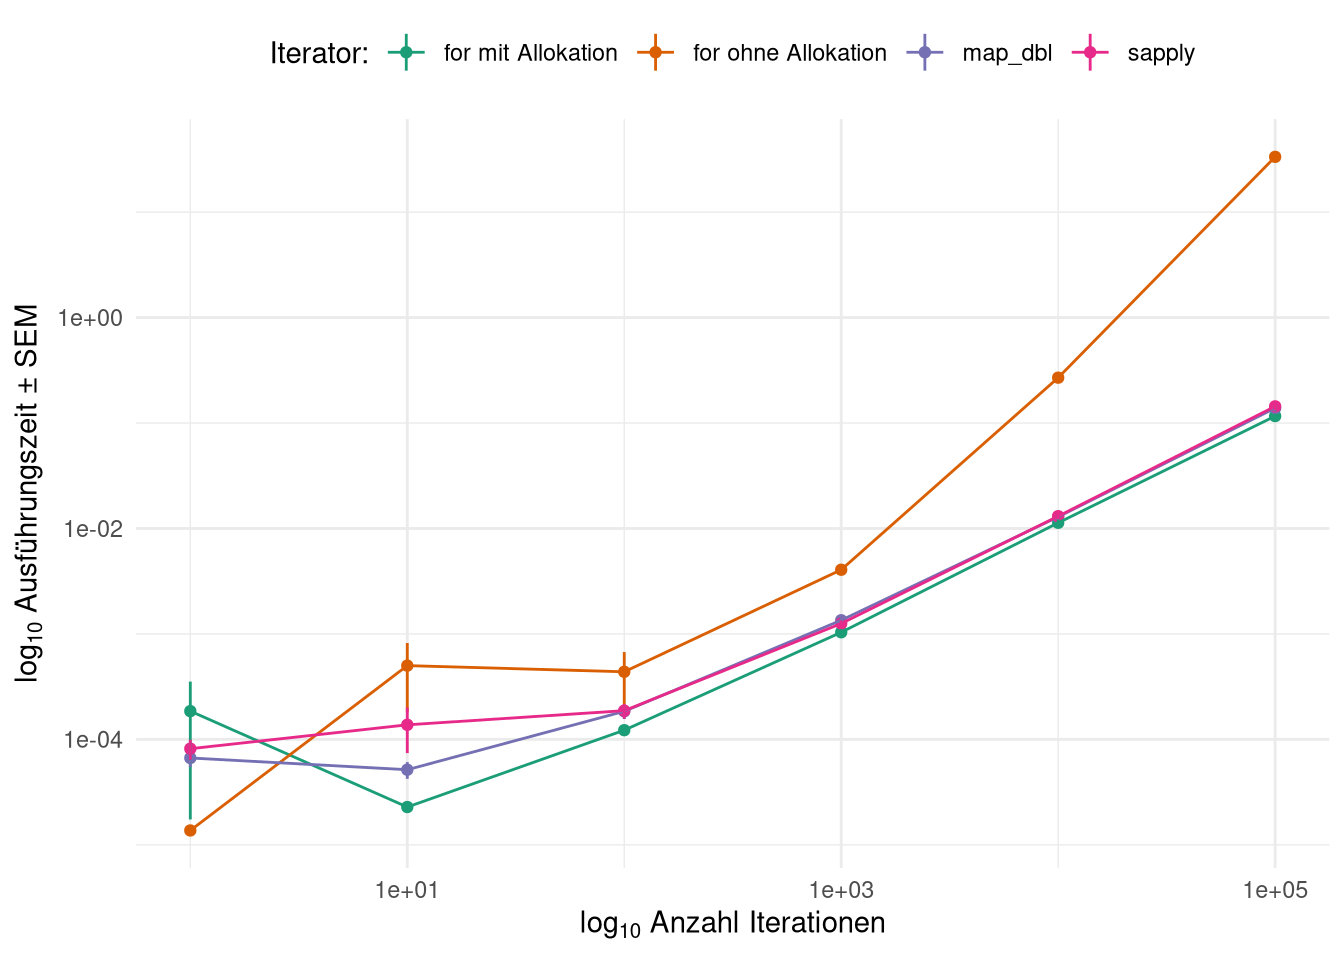
\includegraphics{Robustheit_files/figure-latex/unnamed-chunk-72-1.pdf}

  \bibliography{book.bib}

\end{document}
